\documentclass{ctexbeamer}
\usepackage{verbatim}
\usepackage{graphicx}
\usepackage{amsmath}
\usepackage{mathtools}
\usepackage{multirow,booktabs}
\usepackage{tikz}
%\addtobeamertemplate{block begin}{%
%\setlength{\textwidth}{0.9\textwidth}%
%}{}
\usetikzlibrary{calc,positioning,shapes.misc}
\usetikzlibrary{arrows.meta,graphs,graphdrawing}
%\usetikzlibrary{calc}
\usegdlibrary{layered}
\usepackage{tcolorbox}
\usepackage{empheq}
\newcommand*\widefbox[1]{\fbox{\hspace{1em}#1\hspace{1em}}}
%\usetheme{PaloAlto}
%\usetheme{CambridgeUS}
\usetheme{Berkeley}
\logo{\includegraphics[width=1.55cm,height=1.55cm]{logo.jpg}}
\newcounter{savedenum}
\newcommand*{\saveenum}{\setcounter{savedenum}{\theenumi}}
\newcommand*{\resume}{\setcounter{enumi}{\thesavedenum}}


%\includeonly{Chapter2}
\begin{document}
\begin{frame}
      \title{《微波技术基础》}
      \institute{合肥师范学院\\电子信息与电气工程学院\\Sch.EIEE Hefei Normal University}
      \author{杨晶}
      \date{\today}
      \titlepage
\end{frame}

\begin{frame}{教材}
      《微波技术基础》,廖承恩编,西安电子科技大学出版社,2011.5.
      \begin{figure}
            \centering
            \includegraphics[height=6cm]{jiaocai2}
      \end{figure}
\end{frame}

\begin{frame}{参考文献}
      \bibliographystyle{apalike}
      \nocite{Zhao}
      \nocite{Wu}
      \nocite{Colin}
      \nocite{Liang}
      \bibliography{math}
\end{frame}

\begin{frame}{考核模式}
      \begin{enumerate}
            \item 平时成绩$100$分,占总成绩$50\%$
                  \begin{enumerate}
                        \item 学习态度:$100$分,占$20\%$(考勤 $100$分,占$100\%$)
                        \item 课堂参与:$100$分,占$30\%$(课堂表现,课堂回答问题积极性,$100$分,占$100\%$)
                        \item 平时作业:$100$分,占$50\%$(书面作业$100$分,占$100\%$)
                  \end{enumerate}
            \item 期末考核$100$分,占总成绩$50\%$(期末笔试$100$分,占$100\%$)
      \end{enumerate}
\end{frame}

\documentclass{ctexbeamer}
\usepackage{verbatim}
\usepackage{graphicx}
\usepackage{amsmath}
\usepackage{mathtools}
\usepackage{multirow,booktabs}
\usepackage{tikz}
\usetikzlibrary{positioning}
\usetikzlibrary{calc}
\usepackage{tcolorbox}
\usepackage{empheq}
\newcommand*\widefbox[1]{\fbox{\hspace{1em}#1\hspace{1em}}}
%\usetheme{PaloAlto}
%\usetheme{CambridgeUS}
\usetheme{Berkeley}
\logo{\includegraphics[width=1.55cm,height=1.55cm]{logo.jpg}}
\newcounter{savedenum}
\newcommand*{\saveenum}{\setcounter{savedenum}{\theenumi}}
\newcommand*{\resume}{\setcounter{enumi}{\thesavedenum}}

\begin{document}
\begin{frame}
  \title{《微波技术基础》}
  \institute{Sch.EIEE Hefei Normal University}
  \author{杨晶}
  \date{\today}
  \titlepage
\end{frame}

\begin{frame}{目录}
  \tableofcontents
\end{frame}

\begin{frame}{教材}
  《微波技术基础》,廖承恩编,西安电子科技大学出版社,2011.5.
  \begin{figure}
    \centering
    \includegraphics[height=6cm]{jiaocai}
  \end{figure}
\end{frame}

\begin{frame}{参考文献}
  \bibliographystyle{apalike}
  \nocite{Zhao}
  \nocite{Wu}
  \nocite{Colin}
  \nocite{Liang}
  \bibliography{math}
\end{frame}

\begin{frame}{考核模式}
  \begin{enumerate}
    \item 平时成绩$100$分,占总成绩$50\%$
    \begin{enumerate}
    \item 学习态度:$100$分,占$20\%$(考勤 $100$分,占$100\%$)
    \item 课堂参与:$100$分,占$30\%$(课堂表现,课堂回答问题积极性,$100$分,占$100\%$)
    \item 平时作业:$100$分,占$50\%$(书面作业$100$分,占$100\%$)
    \end{enumerate}
    \item 期末考核$100$分,占总成绩$50\%$(期末笔试$100$分,占$100\%$)
  \end{enumerate}
\end{frame}

\begin{frame}{微波技术基础}
  \begin{description}
    \item[第一章] \textcolor{red}{引论}
    \item[第二章] \textcolor{red}{传输线理论}
    \item[第三章] \textcolor{red}{规则金属波导}
    \item[第四章] \textcolor{red}{微波集成传输线}
    \item[第五章] 毫米波介质波导与光波导
    \item[第六章] \textcolor{red}{微波网络基础}
    \item[第七章] \textcolor{red}{微波谐振器}
    \item[第八章] \textcolor{red}{常用微波元件}
    \item[第九章] 微波铁氧体元件
  \end{description}
\end{frame}

\section{第一章\quad 引论}
\begin{frame}{第一章\quad 引论}
  \begin{enumerate}
    \item 微波及其特点
    \item 微波的应用
    \item 本书的内容框图
    \item 导行波及其一般的传输特性
  \end{enumerate}
\end{frame}

\begin{frame}{近代通信技术的发展}
  \begin{columns}
    \begin{column}{0.35\linewidth}
      \centering
      \includegraphics[height=5cm]{fenghuotai}
    \end{column}
    \begin{column}{0.65\linewidth}
      \centering
      \begin{itemize}
        \item 人类历史上最早的通信手段和现在一样是“无线”的。
        \item 人类通信史上革命性变化,是从把电作为信息载体后发生的。
      \end{itemize}
    \end{column}
  \end{columns}
\end{frame}

\begin{frame}{电报的发明}
  \begin{columns}
    \begin{column}{0.5\linewidth}
      \includegraphics[height=4cm]{dianbao}
    \end{column}
    \begin{column}{0.5\linewidth}
      \begin{itemize}
        \item 电报的发明,拉开了电信时代的序幕,开创了人类利用电来传递信息的历史。
      \end{itemize}
    \end{column}
  \end{columns}
\end{frame}

\begin{frame}{电报的发明}
  \begin{columns}
    \begin{column}{0.5\linewidth}
    \begin{figure}
      \includegraphics[width=3.5cm]{Morse.jpg}
      \caption{莫尔斯 Morse.Samrel Finley.Breese (1791-1872)}\label{Morse}
    \end{figure}
    \end{column}
    \begin{column}{0.5\linewidth}
      \begin{itemize}
        \item 美国画家莫尔斯
        \item 在1835年,第一台电报机问世
      \end{itemize}
    \end{column}
  \end{columns}
\end{frame}

\begin{frame}{电报的发明}
  \begin{itemize}
    \item 莫尔斯成功地利用电流的“通”、“断”和“长断”来代替了人类的文字进行传送,这就是鼎鼎大名的莫尔斯电码。
  \end{itemize}
  \centering
  \includegraphics[width=8cm]{morsecode}
\end{frame}

\begin{frame}{电话的发明}
  \begin{columns}
    \begin{column}{0.35\linewidth}
      \includegraphics[height=6.5cm]{dianhua}
    \end{column}
    \begin{column}{0.65\linewidth}
      \begin{itemize}
        \item 1875年6月2日,被人们作为发明电话的伟大日子而加以纪念,而美国波士顿法院路109号也因此载入史册,至今它的门口仍钉着块铜牌,上面镌有:“1875年6月2日电话诞生在此。”
      \end{itemize}
    \end{column}
  \end{columns}
\end{frame}

\begin{frame}{电话的发明}
  \begin{columns}
    \begin{column}{0.4\linewidth}
    \begin{figure}
      \includegraphics[width=3.2cm]{Bell.png}
      \caption{亚历山大·格拉汉姆·贝尔Alexander Graham Bell (1847 - 1922)}
    \end{figure}
    \end{column}
    \begin{column}{0.6\linewidth}
      \begin{itemize}
        \item 美国发明家和企业家。他获得了世界上第一台可用的电话机的专利权(发明者为意大利人安东尼奥·梅乌奇),创建了贝尔电话公司(AT\&T公司的前身)。其被世界誉为“电话之父”。
      \end{itemize}
    \end{column}
  \end{columns}
\end{frame}

\begin{frame}{电话的发明}
  \begin{columns}
    \begin{column}{0.5\linewidth}
      \includegraphics[width=5.5cm]{Bell2}
    \end{column}
    \begin{column}{0.5\linewidth}
      \begin{itemize}
        \item 贝尔在1892年启用第一条长途电话线——从纽约至芝加哥,长约900里。
      \end{itemize}
    \end{column}
  \end{columns}
\end{frame}

\begin{frame}{电话的发明}
  \begin{columns}
    \begin{column}{0.35\linewidth}
      \includegraphics[width=3.5cm]{pengmingbao}
    \end{column}
    \begin{column}{0.65\linewidth}
      \begin{itemize}
        \item 电话传入我国,是在1881年,英籍电气技师皮晓浦在上海十六铺沿街架起一对露天电话,付36文制钱可通话一次,这是中国的第一部电话。1882年2月,丹麦大北电报公司在上海外滩扬于天路办起我国第一个电话局,用户25家。
        \item 1889年,安徽省安庆州候补知州\textbf{彭名保},自行设计了一部电话,包括自制的五六十种大小零件,称为我国第一部自行设计制造的电话。
      \end{itemize}
    \end{column}
  \end{columns}
\end{frame}

\begin{frame}{电磁波的发现}
  % Electromagnetic wave - black
\begin{tikzpicture}[x=(-15:0.9), y=(90:1.0), z=(-150:1.0),
                    line cap=round, line join=round,
                    axis/.style={black, thick,->},
                    vector/.style={>=stealth,->}]
  \large
  \def\A{1}
  \def\nNodes{5} % use even number
  \def\nVectorsPerNode{8}
  \def\N{\nNodes*40}
  \def\xmax{\nNodes*pi/2*1.01}
  \pgfmathsetmacro\nVectors{(\nVectorsPerNode+1)*\nNodes}

  \def\vE{{\color{blue}\mathbf{E}}}
  \def\vB{{\color{red}\mathbf{B}}}
  \def\vk{\mathbf{\hat{k}}}

  % main axes
  \draw[axis] (0,0,0) -- ++(\xmax*1.1,0,0) node[right] {$x$};
  \draw[axis] (0,-\A*1.4,0) -- (0,\A*1.4,0) node[right] {$y$};
  \draw[axis] (0,0,-\A*1.4) -- (0,0,\A*1.4) node[above left] {$z$};

  % small axes
  \def\xOffset{{(\nNodes-2)*pi/2}}
  \def\yOffset{\A*1.2}
  \def\zOffset{\A*1.2}
  \draw[axis] (\xOffset,\yOffset,-\zOffset) -- ++(\A*0.6,0,0) node[right] {$\vk$};
  \draw[axis] (\xOffset,\yOffset,-\zOffset) -- ++(0,\A*0.6,0) node[right] {$\vE$};
  \draw[axis] (\xOffset,\yOffset,-\zOffset) -- ++(0,0,\A*0.6) node[above left] {$\vB$};

  % equation
  %\node[above right] at (\xOffset,-0.5*\yOffset,4*\zOffset)
  %  {$\begin{aligned}
  %    \vE &= \mathbf{E_0}\sin(\vk\cdot\mathbf{x}-c_0t)\\
  %    \vB &= \mathbf{B_0}\sin(\vk\cdot\mathbf{x}-c_0t)\\
  %    \end{aligned}$};
  %\node[below right] at (\xOffset,-0.5*\yOffset,4*\zOffset)
  %  {$\vE\cdot\vk = 0,\;\; \vB\cdot\vk = 0,\;\; \vB = \frac{1}{c_0}\vk\times\vE$};

  % waves
  \draw[blue,very thick,variable=\t,domain=0:\nNodes*pi/2*1.01,samples=\N]
    plot (\t,{\A*sin(\t*360/pi)},0);
  \draw[red,very thick,variable=\t,domain=0:\nNodes*pi/2*1.01,samples=\N]
    plot (\t,0,{\A*sin(\t*360/pi)});

  % draw vectors
  \foreach \k [evaluate={\t=\k*pi/2/(\nVectorsPerNode+1);
                         \angle=\k*90/(\nVectorsPerNode+1);
                         \c=(mod(\angle,90)!=0);}]
              in {1,...,\nVectors}{
    \if\c1
      \draw[vector,blue!50] (\t,0,0) -- ++(0,{\A*sin(2*\angle)},0);
      \draw[vector,red!50] (\t,0,0) -- ++(0,0,{\A*sin(2*\angle)});
    \fi
  }
\end{tikzpicture}
\begin{itemize}
  \item 自从贝尔发明了电话机,这样人人都能手拿一个“话柄”,和远方的亲朋好友谈天说地了。电报和电话的相继发明,使人类获得了远距离传送信息的重要手段。但是,电信号都是通过金属线传送信息的重要手段。但是,电信号都是通过金属线传送的。线路架设到的地方,信息才能传到,这就大大限制了信息的传播范围,特别是在大海、高山,有没有能让信息\textbf{无线}传播的方法?
\end{itemize}
\end{frame}

\begin{frame}{电磁波的发现}
  \begin{columns}
    \begin{column}{0.35\linewidth}
    \begin{figure}
      \includegraphics[width=3.5cm]{faraday.jpg}
      \caption{迈克尔·法拉第Michael Faraday(1791-1867)}
    \end{figure}
    \end{column}
    \hfill
    \begin{column}{0.65\linewidth}
      \includegraphics[width=4.5cm]{faradayexperiment.jpg}
      \begin{itemize}
        \item 英国物理学家、化学家
        \item 1831年发现电磁感应
      \end{itemize}
    \end{column}
  \end{columns}
\end{frame}

\begin{frame}{电磁波的发现}
  \begin{columns}
    \begin{column}{0.35\linewidth}
      \begin{figure}
        \includegraphics[width=3.5cm]{maxwell.jpg}
        \caption{詹姆斯·克拉克·麦克斯韦James Clerk Maxwell (1831-1879)}
      \end{figure}
    \end{column}
    \begin{column}{0.65\linewidth}
      Maxwell Equations:
      %\begin{equation}
        \begin{align*}
          &\nabla\times\vec E=-\frac{\partial \vec B}{\partial t}\\
          &\nabla\times\vec H=\vec{J} +\frac{\partial \vec D}{\partial t}\\
          &\nabla\cdot\vec{D}=\rho\\
          &\nabla\cdot\vec{B}=0
        \end{align*}
      %\end{equation}
      \begin{itemize}
        \item 英国物理学家。1864年,麦氏发表了电磁场理论,成为人类历史上预言电磁波存在的\textbf{第一人}
      \end{itemize}
    \end{column}
  \end{columns}
\end{frame}

\begin{frame}{电磁波的发现}
  \begin{columns}
    \begin{column}{0.35\linewidth}
      \begin{figure}
        \includegraphics[width=3cm]{hertz.jpg}
        \caption{亨利希·鲁道夫·赫兹(1857 - 1894)}
      \end{figure}
    \end{column}
    \begin{column}{0.65\linewidth}
      \begin{figure}
        \flushright
        \includegraphics[width=2.5cm]{hertzexperiment.jpg}
      \end{figure}
      \begin{itemize}
        \item 德国物理学家,1887年,实验证实了电磁波的存在和传播。成为了近代科学技术史的一座里程碑,为了纪念这位杰出的科学家,电磁波的单位便命名为“赫兹($Hz$)”
        \item 证明了麦克斯韦理论的正确,导致了无线电的诞生,开辟了电子技术的新纪元,标志着从“有线电通信”向“无线电通信”的转折点。也是整个移动通信的发源点,应该说,从这时开始,人类开始进入了无线通信的新领域。
      \end{itemize}
    \end{column}
  \end{columns}
\end{frame}

\subsection{1\quad 微波及其特点}
\begin{frame}{微波及其特点}
  电磁波按波长(或频率)划分,则大致可以把$300MHz - 3000GHz$,(对应空气中波长$\lambda$是$1m - 0.1mm$)这一频段的电磁波称之为微波。它处于超短波和红外光波之间。
\end{frame}

\begin{frame}{微波波段的划分}
  \begin{tabular}{cccc}
    \toprule
    波段代号 & 标称波长/cm & 频率范围/GHz & 波长范围/cm \\
    \midrule
     L & 22 & 1-2 & 30-15 \\
     S & 10 & 2-4 & 15-7.5 \\
     C & 5 & 4-8 & 7.5-3.5 \\
     X & 3 & 8-12 & 3.75-2.5 \\
     Ku & 2 & 12-18 & 2.5-1.67 \\
     K & 1.25 & 18-27 & 1.67-1.11 \\
     Ka & 0.8 & 27-40 & 1.11-0.75 \\
     U & 0.6 & 40-60 & 0.75-0.5 \\
     V & 0.4 & 60-80 & 0.5-0.375 \\
     W & 0.3 & 80-100 & 0.375-0.3 \\
     \bottomrule
  \end{tabular}
\end{frame}

\begin{frame}{Maxwell方程组的物理意义}
  \begin{columns}
    \begin{column}{0.4\linewidth}
      \begin{align*}
        & \nabla\times\vec{E} = -\frac{\partial \vec{B}}{\partial t}\\
        & \nabla\times\vec{H} = \vec{J}+\frac{\partial \vec{D}}{\partial t}
      \end{align*}
    \end{column}
    \begin{column}{0.6\linewidth}
      \begin{itemize}
        \item 这两个方程左边物理量为磁(或电),而右边物理量则为电(或磁)。这中间的等号深刻揭示了电与磁的相互转化,相互依赖,相互对立,共存于统一的电磁波中。正是由于电不断转换为磁,而磁又不断转换成为电,才会发生能量交换和贮存。
      \end{itemize}
    \end{column}
  \end{columns}
\end{frame}

\begin{frame}{电与磁的转换}
  \begin{itemize}
    \item Oersted和Faraday的实验证实了电磁转换,而且还知道了只有动磁才能转化为电。
    \item 还需提到:电磁转换为电磁波的出现提供了可能,但不一定是现实。例如电磁振荡也是典型的电磁转换,但没有引起\textbf{波(Wave)}。
    \item 作为力学类比,电磁转换犹如单摆问题中的动能与势能的转化。
  \end{itemize}
\end{frame}

\begin{frame}{Maxwell方程组的物理意义}
  \begin{itemize}
    \item 进一步研究Maxwell方程两边的运算,从物理上看,运算反映一种作用(Action)。方程左边是空间运算(\textbf{旋度});方程右边是时间运算(\textbf{导数}),中间用等号连接。它深刻揭示了电(或磁)场任一地点的变化会转化为磁(或电)场时间的变化;反过来,场的时间变化也会转化成地点的变化。正是这种空间和时间的相互变化构成了波动的外在形式。用通俗的一句话说:即\textbf{一个地点出现过的事物,过了一段时间又在另一地点出现了}。
  \end{itemize}
\end{frame}

\begin{frame}{Maxwell方程组的物理意义}
  \begin{columns}
    \begin{column}{0.4\linewidth}
      \begin{align*}
        & \nabla\times\vec{H} = j\omega\epsilon\vec{E}+\vec{J}\\
        & \nabla\times\vec{E} = -j\omega\mu\vec{H}
      \end{align*}
    \end{column}
    \begin{column}{0.6\linewidth}
      \textbf{单色波}频域的$Maxwell$方程
    \end{column}
  \end{columns}
\begin{itemize}
  \item $Maxwell$方程还指出:电磁转化有一个重要条件,即频率$\omega$。只有较高的$\omega$才能确保电磁的有效转换,直流情况没有转换。可以这样说,在高频封闭电路才有可能变成开放电路。不过很有意思的是频率越高,越难输出功率,这也是一个有趣的矛盾。
\end{itemize}
\end{frame}

\begin{frame}{Maxwell方程组的物理意义}
  \begin{columns}
    \begin{column}{0.4\linewidth}
      \begin{align*}
        &\nabla\times\vec E=-\frac{\partial \vec B}{\partial t}\\
        &\nabla\times\vec H=\vec{J} +\frac{\partial \vec D}{\partial t}\\
        &\nabla\cdot\vec{D}=\rho\\
        &\nabla\cdot\vec{B}=0
      \end{align*}
    \end{column}
    \begin{column}{0.65\linewidth}
      \begin{itemize}
        \item 在Maxwell方程中还存在另一对矛盾对抗,这就构成了Maxwell方程本质的不对称性。尽管为了找其对称性而一直在探索磁流$\vec{M}$的存在,但到目前为止始终未果。
      \end{itemize}
    \end{column}
  \end{columns}
\end{frame}

\begin{frame}{微波的特点}
  \begin{enumerate}
    \item 微波的两重性\\ 微波的两重性指的是对于尺寸大的物体,如大型建筑物、山谷等它显示出粒子的特点——即似光性或直线性,而对于相对尺寸小的物体,又显示出——波动性或似声性。
    \item 微波与“左邻右舍”的比较\\ 微波的“左邻”是超短波和短波,而它的“右舍”又是红外光波。
    \saveenum
  \end{enumerate}
  \begin{columns}
    \begin{column}{0.43\linewidth}
      \begin{tcolorbox}[colback=green!5,colframe=green!40!black,title=微波与超短波、短波比较]
        微波与超短波、短波相比较大大扩展了通讯通道,开辟了微波通讯和卫星通讯。
      \end{tcolorbox}
    \end{column}
    \begin{column}{0.55\linewidth}
      \begin{tcolorbox}[colback=blue!5,colframe=blue!40!black,title=微波与光波比较]
        微波与光波比较,光通过雨雾衰减很大,特别是雾天,蓝光、紫光几乎看不见,这正是采用红光作警戒的原因。而微波波段穿透力强。
      \end{tcolorbox}
    \end{column}
  \end{columns}
\end{frame}

\begin{frame}{微波的特点}
  \begin{enumerate}
    \resume
    \item 宇宙“窗口”\\地球的外层空间由于日光等繁复的原因形成独特的电离层,它对于短波几乎全反射,这就是短波的天波通讯方式。因而在微波波段则有若干个可以通过电离层的“宇宙窗口”。因而微波是独特的宇宙通讯手段。
    \saveenum
  \end{enumerate}
  \centering
  \includegraphics[width=6.5cm]{cosmicwindow.png}
\end{frame}

\begin{frame}{微波的特点}
  \begin{enumerate}
    \resume
    \item 计算机的运算次数进入十亿次,其频率也是微波频率。超高速集成电路的互耦也是微波互耦问题,因此,微波的研究已进入集成电路和计算机。
    \item 微波研究方法主要有两种:场论的研究方法和网络的研究方法。这也是本门课程要学习的重要方法。其中场论方法的基础是本征模理论。网络方法的基础是广义传输线理论。
  \end{enumerate}
\end{frame}

\subsection{2\quad 微波的应用}
\begin{frame}{微波技术的应用}
  \begin{tikzpicture}
    \node[draw,
    %fill=blue,
    minimum width=2cm,
    minimum height=1.2cm]
    (sum) at (0,0){微波应用};
  \end{tikzpicture}
\end{frame}

\begin{frame}{微波技术的发展}

\end{frame}

\subsection{3\quad 本课程内容}
\begin{frame}{本课程内容}
  \begin{columns}
    \begin{column}{0.15\linewidth}
      \begin{enumerate}
        \item 引论
        \saveenum
      \end{enumerate}
    \end{column}
    \begin{column}{0.35\linewidth}
      \textcolor{blue}{均匀传输线和波导理论基础}\\
      \textcolor{blue}{微波电路元件}
    \end{column}
    \begin{column}{0.5\linewidth}
      \begin{enumerate}
        \resume
        \item \textbf{传输线理论}
        \item \textbf{规则金属波导}
        \item \textbf{微波集成电路}
        \item 毫米波介质波导与光波导
        \item \textbf{微波网络基础}
        \item \textbf{微波谐振器}
        \item \textbf{常用微波器件}
        \item 微波铁氧体元件
      \end{enumerate}
    \end{column}
  \end{columns}
\end{frame}

\begin{frame}{微波技术的研究方法}

\end{frame}

\subsection{4\quad 导行波及其传输特性}
\begin{frame}{基本概念}
  \begin{enumerate}
    \item \textbf{导行系统(Guided system)}
    \saveenum
    \\约束或导引电磁能量定向传播\\
    作用:\\
    \begin{itemize}
      \item 无辐射损耗的将电磁波从一处传到另一处
      \item 设计成微波元件:滤波器、阻抗变换器、定向耦合器等。
    \end{itemize}
    微波电路是一种由各种导行系统构成的导行电磁波电路
  \end{enumerate}

\end{frame}

\begin{frame}{导行系统结构}
  %\begin{figure}
    \centering
    \includegraphics[width=9cm]{guidesystem.png}
  %\end{figure}
\end{frame}

\begin{frame}{基本概念}
  \begin{enumerate}
    \resume
    \item \textbf{导行波(Guided Wave)}
    \\沿导行系统定向传播的电磁波(导波)
    \\\textbf{TEM波}\quad 横电磁波 —— 各种传输线 电磁能量约束或限制在导体之间的空间内沿其轴向传播
    \\\textbf{TE/TM波}\quad 横电/横磁波 —— 封闭金属波导 电磁能量完全限制在金属管内沿轴向传播
    \\\textbf{表面波} —— 开波导 电磁能量约束在波导结构的周围(波导内和波导表面附近)沿轴向传播
    \saveenum
  \end{enumerate}
\end{frame}

\begin{frame}{基本概念}
  \begin{enumerate}
    \resume
    \item \textbf{导模(Guided mode)}
    \\导行波的模式(传输模)
    \\ *在导行系统横截面上的电磁场呈驻波分布,且完全确定的,与位置和频率无关
    \\ *导模是离散的,当频率一定时,每个导模具有唯一的传播常数
    \\ *导模之间相互正交,彼此独立,互不耦合
    \\ *具有截止特性,截止条件和截止波长因导行系统和模式而异
    \item \textbf{规则导行系统(Regular guided system)}
    \\无限长笔直导行系统,其横截面尺寸、媒质分布、结构材料、边界条件沿轴向均不变化
  \end{enumerate}
\end{frame}

\begin{frame}{导波场的分析}
  在\textbf{均匀}、\textbf{无耗}、\textbf{各向同性}、\textbf{无源}导行系统中
  \begin{columns}
    \begin{column}{0.5\linewidth}
      \begin{empheq}[box=\widefbox]{align*}
        &\nabla\times\vec E=-\frac{\partial \vec B}{\partial t}\\
        &\nabla\times\vec H=\vec{J} +\frac{\partial \vec D}{\partial t}\\
        &\nabla\cdot\vec{D}=\rho\\
        &\nabla\cdot\vec{B}=0
      \end{empheq}
      设导波沿$z$向传播,坐标$z$与横向坐标无关
    \end{column}
    \begin{column}{0.5\linewidth}
      \flushright
      \includegraphics[width=4cm]{zuobiao.png}
      \begin{align*}
        & \nabla=\nabla_{t}+\hat z \partial / \partial z\\
        & \vec E=\vec E_{t}+\hat z E_{z}\\
        & \vec H=\vec H_{t}+\hat z H_{z}
      \end{align*}
    \end{column}
  \end{columns}
\end{frame}

\newcommand{\mtikzmark}[1]{\tikz[overlay,remember picture]\node(#1){};}
\tikzset{mylabel/.style={align=center,fill=blue!10,font=\footnotesize}}
%\mytlabel[options]{start.mark}{end.mark}{text}
\newcommand\mytlabel[4][]{%
\tikz[overlay,remember picture]
{\draw[->]([yshift=-10pt]#2.north) -- node[mylabel,#1]{#4}([yshift=6pt]#3.north);}
}
\begin{frame}{导波场的分析}
  \begin{columns}
    \begin{column}{0.45\linewidth}
      \begin{empheq}[box=\widefbox]{align*}
        %\tikzmarkin{c}(0.05,-0.6)(-0.05,0.65)
        & \nabla_t\times\vec{H_{t}}=j\omega\epsilon\hat{z}E_{z} \\
        & \nabla_t\times\hat{z}H_{z}+\hat{z}\times\frac{\partial\vec{H_{t}}}{\partial z}
        = \mtikzmark{a}j\omega\epsilon\vec{E_{t}}
      \end{empheq}
      %$$\times j\omega\mu$$
    \end{column}
    \begin{column}{0.5\linewidth}
      \begin{empheq}[box=\widefbox]{align*}
        & \nabla_t\times\vec E_{t}=-j\omega\mu\hat{z} H_{z} \\
        & \nabla_t\times \hat z E_{z}+\hat{z}\times\mtikzmark{c}\frac{\partial\vec{E_{t}}}{\partial z}
        = -j\omega\mu\vec{H_t}
      \end{empheq}
    \end{column}
  \end{columns}
  \begin{flalign*}
      & j\omega\mu\hat{z}\times\frac{\partial \vec{H_{t}}}{\partial z}=\mtikzmark{b}-j\omega\mu\nabla_{t}\times\hat{z}H_{z}-\omega^{2}\mu\epsilon\vec{E_{t}} &
  \end{flalign*}
  \begin{flalign*}
    && -j\omega\mu\hat{z}\times\frac{\partial \vec{H_{t}}}{\partial z}=\hat{z}\times\frac{\partial}{\partial z} \left(\nabla_{t}\times\hat{z}E_{z}\right)+\hat{z}\times\mtikzmark{d}\frac{\partial}{\partial z} \left(\hat{z} \times \frac{\partial \vec{E_{t}}}{\partial z} \right)
  \end{flalign*}
  % draw arrow with text from specified position to another
  \mytlabel{a}{b}{$\times j\omega\mu$}
  \mytlabel{c}{d}{$\hat{z}\times\frac{\partial}{\partial z}$}
\end{frame}

\begin{frame}{导波场的分析}
  \begin{empheq}[box=\widefbox]{align*}
    \left( k^{2}+\frac{\partial^{2}}{\partial z^{2}} \right)\vec{E_{t}}=\frac{\partial}{\partial z}\nabla_{t}E_{z}-j\omega\mu\nabla_{t}\times\hat{z}H_{z}
  \end{empheq}
  \begin{empheq}[box=\widefbox]{align*}
    \left( k^{2}+\frac{\partial^{2}}{\partial z^{2}} \right)\vec{H_{t}}=\frac{\partial}{\partial z}\nabla_{t}H_{z}-j\omega\epsilon\nabla_{t}\times\hat{z}E_{z}
  \end{empheq}
  在规则导行系统中,导波场的\textbf{横向分量}可用\textbf{纵向分量}完全确定。\\上面公式中$k^{2}=\omega^{2}\mu\epsilon$
\end{frame}

\begin{frame}{导波场的分析}
  \begin{empheq}[box=\widefbox]{align*}
    & \nabla^{2}\vec{E}+k^{2}\vec{E}=0\\
    & \nabla^{2}\vec{H}+\mtikzmark{a}k^{2}\vec{H}=0
  \end{empheq}
  \begin{columns}
    \begin{column}{0.45\linewidth}
      \begin{empheq}[box=\widefbox]{align*}
        & \nabla^{2}E_{z}+\mtikzmark{b}k^{2}E_{z}=0\\
        & \nabla^{2}H_{z}+\mtikzmark{d}k^{2}H_{z}=0
      \end{empheq}
    \end{column}
    \begin{column}{0.45\linewidth}
      \begin{empheq}[box=\widefbox]{align*}
        & \nabla^{2}\vec{E}_{t}+\mtikzmark{c}k^{2}\vec{E}_{t}=0\\
        & \nabla^{2}\vec{H}_{t}+k^{2}\vec{H}_{t}=0
      \end{empheq}
    \end{column}
  \end{columns}
  \flushright
  \begin{empheq}[box=\widefbox]{align*}
    \left( \nabla^{2}_{t}+\frac{\partial^{2}}{\partial z^{2}}\right)
    \left\{\begin{aligned}
      \mtikzmark{e}E_{z}(z,t)\\H_{z}(z,t)
    \end{aligned}\right\}
    +k^{2}
    \left\{\begin{aligned}
      E_{z}(z,t)\\H_{z}(z,t)
    \end{aligned}\right\}
    =0
  \end{empheq}
  \mytlabel{a}{b}{纵向场}
  \mytlabel{a}{c}{横向场}
  \mytlabel{d}{e}{Helmholtz Equation}
\end{frame}

\begin{frame}{导波场的分析}
  \begin{empheq}[box=\widefbox]{align*}
    \left( \nabla^{2}_{t}+\frac{\partial^{2}}{\partial z^{2}}\right)
    \left\{\begin{aligned}
      \mtikzmark{e}E_{z}(z,t)\\H_{z}(z,t)
    \end{aligned}\right\}
    +k^{2}
    \left\{\begin{aligned}
      E_{z}(z,t)\\H_{z}(z,t)
    \end{aligned}\right\}
    =0
  \end{empheq}
  \begin{enumerate}
    \item \textbf{分离变量法}\\
    令$E_{z}(z,t)=Z(z)E_{0z}(t)$ \\
    \begin{align*}
      \frac{\nabla_{t}^{2}E_{0z}(t)}{E_{0z}(t)}+\frac{d^{2}Z(z)/dz^{2}}{Z(z)}=-k^{2}
    \end{align*}
    \begin{columns}
      \begin{column}{0.3\linewidth}
        分离变量常数: $k_{c}$和$\beta$
      \end{column}
      \begin{column}{0.6\linewidth}
        \begin{empheq}[box=\widefbox]{align*}
          & d^{2}Z(z)/dz^{2}+\beta^{2}Z(z)=0 \\
          & \nabla_{t}^{2}E_{0z}(t)+k_{c}^{2}E_{0z}(t)=0
        \end{empheq}
        \flushright————本征值方程
      \end{column}
    \end{columns}
    \saveenum
  \end{enumerate}
\end{frame}

\begin{frame}{导波场的分析}
  \begin{enumerate}
    \resume
    \item \textbf{色散关系}
    \begin{columns}
      \begin{column}{0.55\linewidth}
        \begin{empheq}[box=\widefbox]{align*}
          & k^{2}=k_{c}^{2}+\beta^{2}\\
          & \beta=\sqrt{k^{2}-k_{c}^{2}}=k\sqrt{1-(k_{c}/k)^{2}}
        \end{empheq}
      \end{column}
      \begin{column}{0.4\linewidth}
        \raggedright
        $k^{2}=\omega^{2}\mu\epsilon$\\  $\beta$:导波的传播常数或相移常数
      \end{column}
    \end{columns}
    $$d^{2}Z(z)/dz^{2}+\beta^{2}Z(z)=0$$
    %\flushleft
    解:
    \begin{empheq}[box=\widefbox]{align*}
      Z(z)=A_{1}exp(-j\beta z)+A_{2}exp(j\beta z)
    \end{empheq}
    规则导行系统中沿正$z$方向传播的导波纵向场分量\\
    \begin{align*}
      E_{z}(t,z)=E_{0z}(t)exp(-j\beta z)\\
      H_{z}(t,z)=H_{0z}(t)exp(-j\beta z)
    \end{align*}
    \saveenum
  \end{enumerate}
\end{frame}

\begin{frame}{导波场的分析}
  \begin{enumerate}
    \resume
    \item 本征值方程
    \begin{empheq}[box=\widefbox]{align*}
      \nabla_{t}^{2}E_{0z}(t)+k_{c}^{2}E_{0z}(t)=0
    \end{empheq}
    $k_{c}$:在特定边界条件下的本征值,称为导波的横向截止波数\\
    $k_{c}\neq 0$
    \saveenum
  \end{enumerate}
\end{frame}

\begin{frame}{导波场的分析}
  \begin{enumerate}
    \resume
    \item 横-纵向场的关系
    \begin{empheq}[box=\widefbox]{align*}
      \left( k^{2}+\frac{\partial_{2}}{\partial z^{2}}\right)\vec{E}_{t}=\frac{\partial}{\partial z}\nabla_{t}E_{z}-j\omega\mu\nabla_{t}\times\hat{z}H_{z}\\
      \left( k^{2}+\frac{\partial_{2}}{\partial z^{2}}\right)\vec{H}_{t}=\frac{\partial}{\partial z}\nabla_{t}H_{z}-j\omega\epsilon\nabla_{t}\times\hat{z}E_{z}
    \end{empheq}
    \begin{columns}
      \begin{column}{0.6\linewidth}
        \begin{empheq}[box=\widefbox]{align*}
          \vec{E}_{t}=\frac{-j\beta}{k_{c}^{2}}\left[\nabla_{t}E_{z}+Z_{h}\nabla_{t}H_{z}\times\hat{z}\right]\\
          \vec{H}_{t}=\frac{-j\beta}{k_{c}^{2}}\left[\nabla_{t}H_{z}+Y_{e}\hat{z}\times\nabla_{t}E_{z}\right]
        \end{empheq}
      \end{column}
      \begin{column}{0.4\linewidth}
        \begin{align*}
          Z_{h}=\sqrt{\frac{\mu}{\epsilon}}\frac{k}{\beta}\\
          Y_{e}=\sqrt{\frac{\epsilon}{\mu}}\frac{k}{\beta}
        \end{align*}
      \end{column}
    \end{columns}
    \saveenum
  \end{enumerate}
\end{frame}

\begin{frame}{导波场的分析}
  \begin{enumerate}
    \resume
    \item 导波的种类\\
    横磁波(TM)或电(E)波——
    \begin{empheq}[box=\widefbox]{align*}
      H_{z}=0
    \end{empheq}
    \begin{columns}
      \begin{column}{0.4\linewidth}
        \begin{empheq}[box=\widefbox]{align*}
          \vec{E}_{t}^{e}=\frac{-j\beta}{k_{c}^{2}}\nabla_{t}E_{z}
        \end{empheq}
      \end{column}
      \begin{column}{0.6\linewidth}
        \begin{empheq}[box=\widefbox]{align*}
          \vec{H}_{t}^{e}=\frac{-j\beta}{k_{c}^{2}}Y_{e}\hat{z}\times\nabla_{t}E_{z}
        \end{empheq}
      \end{column}
    \end{columns}

  \end{enumerate}
\end{frame}

\begin{frame}{导波场的分析}

\end{frame}

\begin{frame}{导波场的分析}

\end{frame}

\begin{frame}{导波场的分析}

\end{frame}

\begin{frame}{导行波的一般传输特性}

\end{frame}

\begin{frame}{导行波的一般传输特性}

\end{frame}

\begin{frame}{导行波的一般传输特性}

\end{frame}

\begin{frame}{导行波的一般传输特性}

\end{frame}

\end{document}

\section{第2章\quad 从低频电路到微波分析}
\begin{frame}
    通常电路分析应用于元件尺寸远小于工作波长、电路中的各元件(如电阻、电容和电感)彼此独立、位置固定的低频电路。这意味着在所讨论的频率范围内,基本电路元件电阻 $R$ 、电容 $C$ 和电感 $L$ 在各自所处的区域内将分别表现为电阻消耗能量、电容存储电能、
    电感产生磁场,低频电路的上述条件使得我们可将低频电路中的所有元件都视为集总元件。而在微波频段这些电路元件不再表现为纯电阻、电容和电感,而是有额外的阻抗和电抗(寄生效应)。在微波频段,同一元件在不同频率下可能会表现出不同的容性、感性或阻性。
\end{frame}

\subsection{基本电路元件}
\begin{frame}{基本电路元件}{电阻$R$}
    \begin{columns}
        \begin{column}{0.3\linewidth}
            \centering
            $I=\frac{V}{R}$
        \end{column}
        \begin{column}{0.7\linewidth}
            \begin{circuitikz}
                \draw (0,0)
                to[V,v=$V$] (0,2)
                to[short] (5,2)
                to[R=$R$] (5,0)
                to[short] (0,0);
                \draw[->] (2,2.2) -- (3,2.2);
                \draw (2.4,2.2) node[anchor=south] {$I$};
            \end{circuitikz}
        \end{column}
    \end{columns}
    \begin{columns}
        \begin{column}{0.5\linewidth}
            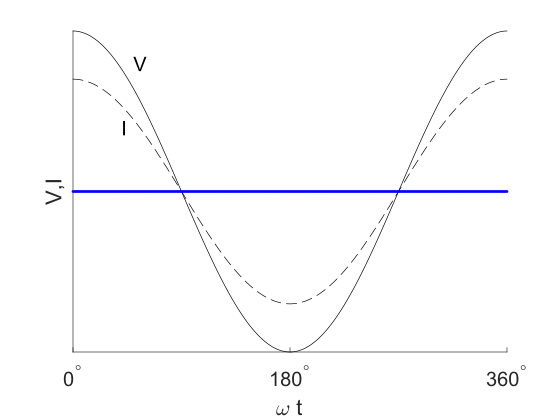
\includegraphics[width=5cm]{Cha2//fig2_1.eps}
        \end{column}
        \begin{column}{0.5\linewidth}
            \tikzset{help lines/.style=thin}
            \tikzset{Karl's grid/.style={help lines,color=blue!50}}
            \begin{tikzpicture}[scale=3]
                \draw (-0.9,0) -- (0.9,0);
                \draw (0,-0.5) -- (0,0.5);
                \draw[red,thick,->] (0,0) -- (0.4,0);
                \draw[blue,thick,->] (0,0) -- (0.7,0);
                \draw (-0.9,0) node[anchor=north] {$180^{\circ}$};
                \draw (0.9,0) node[anchor=north] {$0^{\circ}$};
                \draw (0,-0.5) node[anchor=west] {$270^{\circ}$};
                \draw (0,0.5) node[anchor=west] {$90^{\circ}$};
                \draw (0.4,0) node[anchor=north] {$I$};
                \draw (0.7,0) node[anchor=north] {$V$};
            \end{tikzpicture}
        \end{column}
    \end{columns}
\end{frame}

\begin{frame}{基本电路元件}{电感$L$}
    \begin{columns}
        \begin{column}{0.3\linewidth}
            \begin{align*}
                 & v(t)=L\frac{\mathrm{d} i(t)}{\mathrm{d}t} \quad i(t)=\frac{1}{L}\int_0^t v(t)\mathrm{d}t \\
                 & v(t)=V_0\cos \omega t                                                                    \\
                 & I = \frac{1}{L}\int V_0\cos\omega t \mathrm{d}t=\frac{V_0\sin\omega t}{\omega L}
            \end{align*}
        \end{column}
        \begin{column}{0.7\linewidth}
            \begin{circuitikz}
                \draw (0,0)
                to[V,v=$V$] (0,2)
                to[short] (5,2)
                to[L=$L$] (5,0)
                to[short] (0,0);
                \draw[->] (2,2.2) -- (3,2.2);
                \draw (2.4,2.2) node[anchor=south] {$I$};
            \end{circuitikz}
        \end{column}
    \end{columns}
    \begin{columns}
        \begin{column}{0.5\linewidth}
            \includegraphics[width=5cm]{Cha2//fig2_2.eps}
        \end{column}
        \begin{column}{0.5\linewidth}
            \tikzset{help lines/.style=thin}
            \tikzset{Karl's grid/.style={help lines,color=blue!50}}
            \begin{tikzpicture}[scale=3]
                \draw (-0.9,0) -- (0.9,0);
                \draw (0,-0.5) -- (0,0.5);
                \draw[red,thick,->] (0,0) -- (0,-0.4);
                \draw[blue,thick,->] (0,0) -- (0.7,0);
                \draw (-0.9,0) node[anchor=north] {$180^{\circ}$};
                \draw (0.9,0) node[anchor=north] {$0^{\circ}$};
                \draw (0,-0.5) node[anchor=west] {$270^{\circ}$};
                \draw (0,0.5) node[anchor=west] {$90^{\circ}$};
                \draw (0,-0.4) node[anchor=west] {$I$};
                \draw (0.7,0) node[anchor=north] {$V$};
            \end{tikzpicture}
        \end{column}
    \end{columns}
\end{frame}

%\begin{comment}
\begin{frame}{基本电路元件}{电容$C$}
    \begin{columns}
        \begin{column}{0.3\linewidth}
            \begin{align*}
                 & i(t)=C \frac{\partial v(t)}{\partial t} \quad v(t)=\frac{1}{C}\int_0^t i(t)\mathrm{d}t \\
                 & v(t)=V_0\cos \omega t                                                                    \\
                 & I = C \frac{\partial v(t)}{\partial t}=-V_0\omega C\sin\omega t
            \end{align*}
        \end{column}
        \begin{column}{0.7\linewidth}
            \begin{circuitikz}
                \draw (0,0)
                to[V,v=$V$] (0,2)
                to[short] (5,2)
                to[C=$C$] (5,0)
                to[short] (0,0);
                \draw[->] (2,2.2) -- (3,2.2);
                \draw (2.4,2.2) node[anchor=south] {$I$};
            \end{circuitikz}
        \end{column}
    \end{columns}
    \begin{columns}
        \begin{column}{0.5\linewidth}
            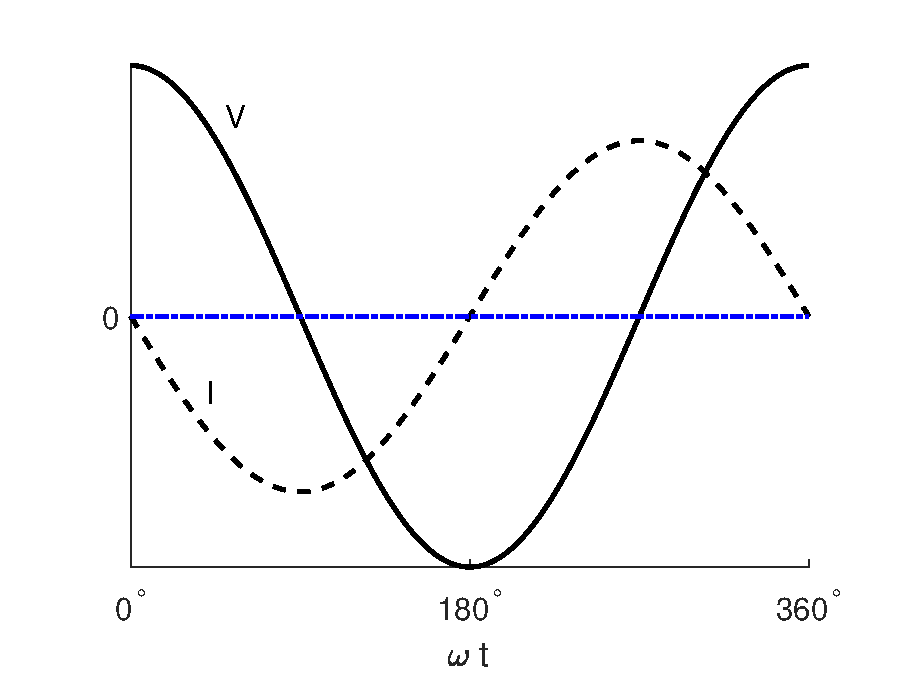
\includegraphics[width=5cm]{Cha2//fig2_3.eps}
        \end{column}
        \begin{column}{0.5\linewidth}
            \tikzset{help lines/.style=thin}
            \tikzset{Karl's grid/.style={help lines,color=blue!50}}
            \begin{tikzpicture}[scale=3]
                \draw (-0.9,0) -- (0.9,0);
                \draw (0,-0.5) -- (0,0.5);
                \draw[red,thick,->] (0,0) -- (0,0.4);
                \draw[blue,thick,->] (0,0) -- (0.7,0);
                \draw (-0.9,0) node[anchor=north] {$180^{\circ}$};
                \draw (0.9,0) node[anchor=north] {$0^{\circ}$};
                \draw (0,-0.5) node[anchor=west] {$270^{\circ}$};
                \draw (0,0.5) node[anchor=west] {$90^{\circ}$};
                \draw (0,0.4) node[anchor=west] {$I$};
                \draw (0.7,0) node[anchor=north] {$V$};
            \end{tikzpicture}
        \end{column}
    \end{columns}
\end{frame}
%\end{comment}

\subsection{电压和电流相量}
\begin{frame}{电压和电流相量}
    相量电压 $V$ 来表示正弦电压 $v(t)$ ; 相量电流 $I$ 来表示产生的电流 $i(t)$
    \begin{align*}
         & v(t)=\mathrm{Re}[V\mathrm{e}^{\mathrm{j}\omega t}] \\
         & i(t)=\mathrm{Re}[I\mathrm{e}^{\mathrm{j}\omega t}]
    \end{align*}
    $L$ 和 $C$ 元件的电抗是单位为 $\Omega$ 的正实数
    $$X_L = \omega L(\Omega) \quad X_C = \frac{1}{\omega C}(\Omega)$$
    阻抗
    \begin{align*}
        & Z_L=\mathrm{j} \omega L \quad Z_C=-\mathrm{j} \frac{1}{\omega C} \\
        & Z=R+\mathrm{j} (X_L-X_C)=R+\mathrm{j} (\omega L-1/\omega C)
   \end{align*}
\end{frame}

\subsection{阻抗和导纳}
\begin{frame}{阻抗和导纳}
$$X_L=\omega L, \omega=2\pi f$$
频率为$1GHz$,一个 $1nH$ 的电感电抗值为$6.28\Omega$,这样,在其他频率下的其他电感的电抗值为
$$X_L=6.28fL\text{(f的单位GHz,L的单位nH)}$$
同理
$$X_C=\frac{1}{\omega C}, \omega=2\pi f$$
频率为$1GHz$,一个 $1pF$ 的电容电抗值为$159\Omega$,这样,在其他频率下的其他电容的电抗值为
$$X_C=159/fC\text{(f的单位GHz,C的单位pF)}$$
串联阻抗相加
\begin{align*}
    &Z_1=a+\mathrm{j} b \quad Z_2=c+\mathrm{j} d\\
    &Z_T=Z_1+Z_2=(a+c)+\mathrm{j} (b+d)
\end{align*}
\end{frame}

\begin{frame}{阻抗和导纳}
    $$B_L=\frac{1}{X_L}=\frac{1}{\omega L}$$
    电感的导纳为
    $$-\mathrm{j} B_L=\frac{1}{\mathrm{j} X_L}=\frac{1}{\mathrm{j} \omega L}=\frac{-\mathrm{j} }{\omega L}$$
    同理
    $$B_C=\frac{1}{X_C}=\frac{1}{1/\omega C}=\omega C$$
    电容的导纳为
    $$\mathrm{j} B_C=\frac{1}{-\mathrm{j} X_C}=\frac{1}{-\mathrm{j} /\omega C}=\mathrm{j} \omega C$$
    并联导纳相加
    \begin{align*}
        &Z_T=\frac{1}{Y_T}=\frac{1}{Y_1+Y_2}
    \end{align*}
    \end{frame}

\subsection{电路分析基本定律}
\begin{frame}{电路分析基本定律}
    \begin{columns}
        \begin{column}{0.5\linewidth}
            \centering
            \begin{tikzpicture}
                \filldraw[fill=green!50!white] (0,0) circle [radius=1mm];
                \draw[->] (2cm,1cm) -- ({1mm*cos(40)},{1mm*sin(40)});
                \draw ({1.5cm*cos(40)},{1.5cm*sin(40)}) node {$i_2$};
                \draw[->] (-1cm,2cm) -- ({1mm*cos(120)},{1mm*sin(120)});
                \draw ({1.5cm*cos(110)},{1.5cm*sin(110)}) node {$i_1$};
                \draw[->] ({2.24cm*cos(230)},{2.24cm*sin(230)}) -- ({1mm*cos(230)},{1mm*sin(230)});
                \draw ({1.5cm*cos(237)},{1.5cm*sin(237)}) node {$i_n$};

                \foreach \x in {250,275,300,325,350,15}
                \filldraw[fill=green!20!white] ({1.5cm*cos(\x)},{1.5cm*sin(\x)}) circle [radius=0.5mm];
            \end{tikzpicture}
        \end{column}
        \begin{column}{0.5\linewidth}
            \centering
            $$\sum_{n=1}^N i_n(t)=0$$
        \end{column}
    \end{columns}

    \begin{columns}
        \begin{column}{0.8\linewidth}
            \begin{circuitikz}
                \centering
                \draw (0,0) to[R,o-o] (0,3)
                to[short,o-o] (2,3)
                to[R] (5,3)
                to[short,-o] (6,3)
                to[R,-o] (6,0);
                \draw[dashed] (6,0) to[short,o-o] (4,0);
                \draw (4,0) to[R,o-] (1,0);
                \draw[dashed] (1,0) to[short,-o] (0,0);
                \draw[dashed] (2,3) to[short] (2,1.5);
                \draw (4,0) to[short] (4,1.5);
                \draw[dashed] (4,1.5) to[short] (4,2.5);
                
                \draw (6,3) -- (6.5,3);
                \draw[dashed] (6.5,3) -- (8,3);
                \draw (6,0) -- (6.5,0);
                \draw[dashed] (6.5,0) -- (8,0);
                \draw (0,3) -- (-0.5,3);
                \draw[dashed] (-0.5,3) -- (-2,3);
                \draw (0,0) -- (-0.5,0);
                \draw[dashed] (-0.5,0) -- (-2,0);

                \draw(-0.5,2.5) node[anchor=east] {+};
                \draw(-0.5,0.5) node[anchor=east] {-};
                \draw(-0.5,1.5) node[anchor=east] {$v_M$};

                \draw(6.5,2.5) node[anchor=west] {+};
                \draw(6.5,0.5) node[anchor=west] {-};
                \draw(6.5,1.5) node[anchor=west] {$v_2$};

                \draw(2.5,3.2) node[anchor=south] {+};
                \draw(4.5,3.2) node[anchor=south] {-};
                \draw(3.5,3.2) node[anchor=south] {$v_1$};

                \draw(1.5,0.2) node[anchor=south] {-};
                \draw(3.5,0.2) node[anchor=south] {+};
                \draw(2.5,0.2) node[anchor=south] {$v_m$};
            \end{circuitikz}
        \end{column}
        \begin{column}{0.2\linewidth}
            \centering
            $$\sum_{m=1}^M v_m(t)=0$$
        \end{column}
    \end{columns}
\end{frame}

\begin{frame}{电路分析基本定律}
    \centering
    \begin{tabular}{ccc}
        \toprule
         名称 & 时域                                 & 频域                      \\
        \midrule
         电容 & $i(t)=C\mathrm{d}v(t)/\mathrm{d}t$   & $I=\mathrm{j}\omega CV$ \\
         电感 & $v(t)=L\mathrm{d}i(t)/\mathrm{d}t$   & $V=\mathrm{j}\omega LI$ \\
         欧姆定律 & $v(t)=Ri(t)$                     & $V=RI$                   \\
         广义欧姆定律 & $v(t)=Ri+\frac{1}{C} \int_0^t i\mathrm{d}t+L\mathrm{d}i/\mathrm{d}t$ & \makecell{$V(\omega)=Z(\omega)I(\omega)$ \\ $Z=R+\mathrm{j}(\omega L-1/\omega C)$} \\ % 表格内换行
         KCL & $\sum\limits_{n=1}^N i_n(t)=0$       & $\sum\limits_{n=1}^N I_n(\omega)=0$ \\
         KVL & $\sum\limits_{m=1}^M v_m(t)=0$       & $\sum\limits_{m=1}^M V_m(\omega)=0$ \\
        \bottomrule
    \end{tabular}
\end{frame}

\subsection{正弦稳态条件下的功率计算}
\begin{frame}{正弦稳态条件下的功率计算}
    \centering
    \tikzset{
        rect1/.style = {
                shape = rectangle, % 指定样式
                minimum height = 2cm,
                minimum width = 3cm,
                align = center, % 文字居中
            }
    }
    \begin{tikzpicture}
        \node (a) [rect1,draw=black,text width=2cm] {源或信号发生器};
        \node[right of=a,xshift=100pt] (b) [rect1,draw=black,text width=2cm] {线性负载网络$N$};
        \draw (1.5cm,0.5cm) -- (2.2cm,0.5cm);
        \draw (2.3cm,0.5cm) -- (3cm,0.5cm);
        \draw (1.5cm,-0.5cm) -- (2.2cm,-0.5cm);
        \draw (2.3cm,-0.5cm) -- (3cm,-0.5cm);
        \draw (2.25cm,0.5cm) circle [radius=0.5mm];
        \draw (2.25cm,-0.5cm) circle [radius=0.5mm];
        \draw[->] (2cm,-1cm) -- (2cm,-0.1cm) -- (2.4cm,-0.1cm);
        \draw (2cm,-1cm) node[anchor=north] {$Z,Y$};
        \draw[->] (2.4cm,0.75cm) -- (2.8cm,0.75cm);
        \draw (2.4cm,0.75cm) node[anchor=south] {$i(t)$};
        \draw (2.25cm,0.6cm) node[anchor=north] {$+$};
        \draw (2.25cm,-0.63cm) node[anchor=south] {$-$};
    \end{tikzpicture}\\
    \begin{columns}
        \begin{column}{0.5\linewidth}
            \centering
            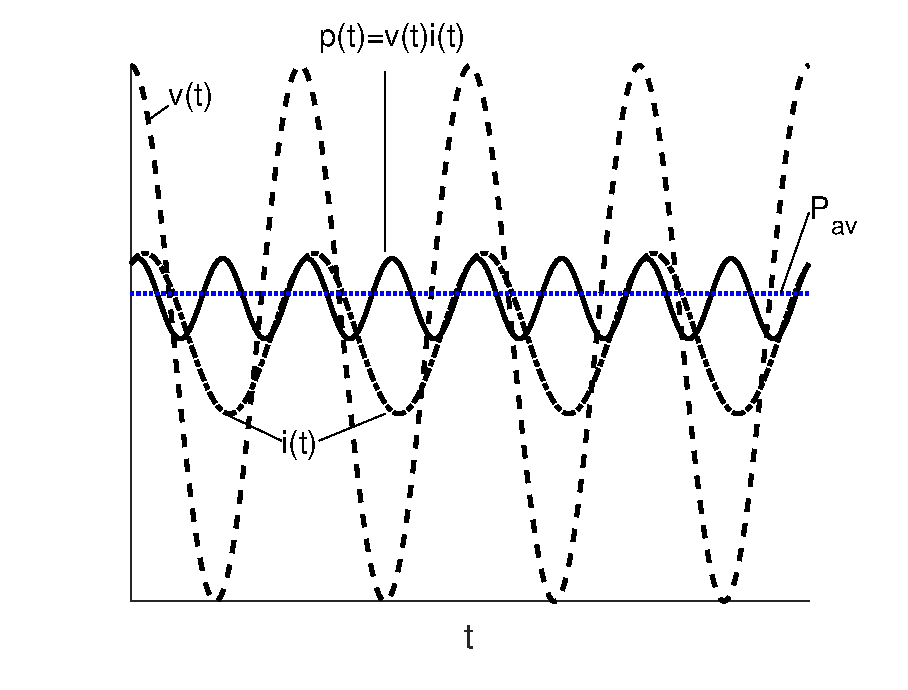
\includegraphics[width=5cm]{Cha2//fig2_8.eps}
        \end{column}
        \begin{column}{0.5\linewidth}
            瞬时功率:$p(t)=v(t)i(t)$ \\
            平均功率:$P_{av}=\dfrac{1}{T}{\displaystyle \int_0^T}p(t)\mathrm{d}t=\dfrac{1}{T}{\displaystyle \int_0^T}v(t)i(t)\mathrm{d}t$\\
            复功率:$P=\dfrac{1}{2}VI^*$
        \end{column}
    \end{columns}
\end{frame}

\subsection{分贝}
\begin{frame}{分贝}
\begin{align*}
    &N(\mathrm{dB})=10\lg(P_2/P_1)\\
    &\text{分贝瓦}(\mathrm{dBW}):N(\mathrm{dBW})=10\lg(P_2/1\mathrm{W})\\
    &\text{分贝毫瓦}(\mathrm{dBmW}):N(\mathrm{dBmW})=10\lg(P_2/1\mathrm{mW})\\
    &\text{分贝微瓦}(\mathrm{dB\mu W}):N(\mathrm{dB\mu W})=10\lg(P_2/1\mathrm{\mu W})
\end{align*}
奈培$(Np)$:奈培定义为两个电流、电压或场强的比值的自然对数(以$e$为底的对数),它是表征衰减的单位。如果电压从$V_1$衰减至$V_2$,则有\\
\begin{align*}
    &V_2/V_1=e^{-N}\\
    &N(\mathrm{Np})=\ln(V_2/V_1)^{-1}=-\ln(V_2/V_1)\\
    &1\mathrm{Np}=-\ln(V_2/V_1)\Rightarrow V_2/V_1=1/\mathrm{e}\\
    &1\mathrm{Np}=20\lg[1/(V_2/V_1)]=20\lg\mathrm{e}=8.686\mathrm{dB}
\end{align*}
\end{frame}

\subsection{趋肤效应}
\begin{frame}{趋肤效应}
    \begin{columns}
        \begin{column}{0.6\linewidth}
            \centering
            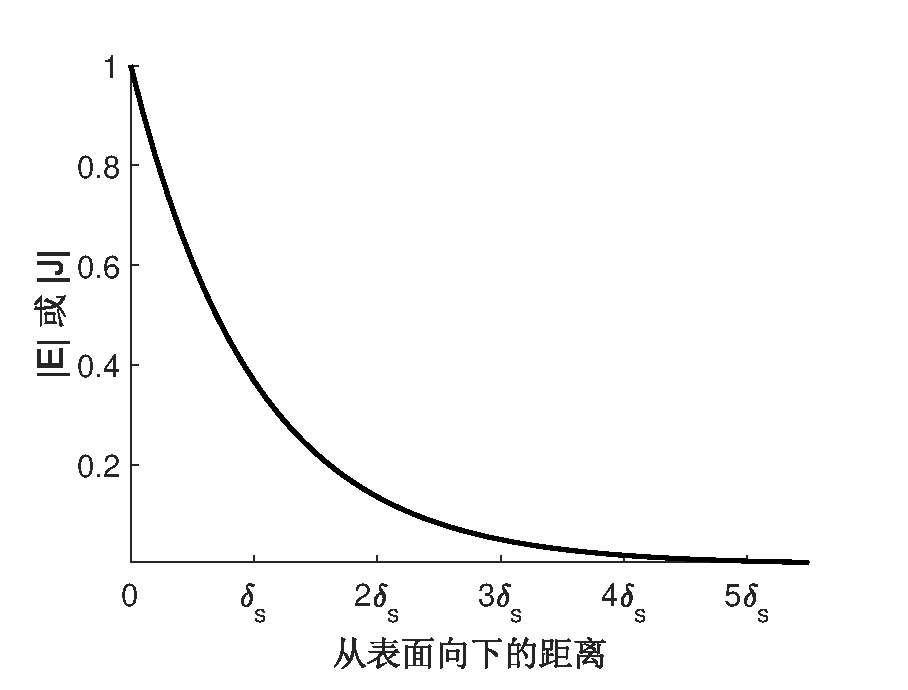
\includegraphics[width=6cm]{Cha2//fig2_9.eps}
        \end{column}
        \begin{column}{0.4\linewidth}
            \centering
            \begin{align*}
                &\vec J = \sigma \vec E\\
                &\vec J = \vec J_0 \mathrm{e}^{-z/\delta_s}\\
                &\delta_s = \frac{1}{\sqrt{\pi f\mu\sigma}}\\
                & R_{AC} = \frac{1}{\pi D\delta_S\sigma} \\
                & R_{DC} = \frac{1}{\pi(D^2/4)\sigma}
            \end{align*}
        \end{column}
    \end{columns}

\end{frame}
\section{第三章\quad 规则金属波导}
\begin{frame}{第三章\quad 规则金属波导}

\end{frame}

\subsection{矩形波导}
\begin{frame}{矩形波导}

\end{frame}

\subsection{圆形波导}
\begin{frame}{圆形波导}

\end{frame}

\subsection{同轴线}
\begin{frame}{同轴线}

\end{frame}

\subsection{波导正交模的特性}
\begin{frame}{波导正交模的特性}

\end{frame}

\subsection{波导的激励}
\begin{frame}{波导的激励}

\end{frame}

\section{第4章\quad Smith圆图与阻抗匹配}
\begin{frame}
  Smith圆图是1939年由Phillip Smith在贝尔电话实验室工作时开发的,Smith圆图全面反映了反射系数与阻抗/导纳之间的相互换算关系,求解传输线问题是非常有用的。主要用在以下方面:
  \begin{itemize}
    \item 无耗传输线的分析
    \item 传输线的阻抗匹配
  \end{itemize}
\end{frame}

\subsection{Smith圆图}
\begin{frame}{Smith圆图的基本构成}
  上一章分析都是围绕如下公式及相互关系展开的:
  \begin{empheq}[box=\widefbox]{align*}
    Z_{in}(d)=\frac{V_L\cosh\gamma d+I_LZ_0\sinh\gamma d}{I_L\cosh\gamma d+\dfrac{V_L\sinh\gamma d}{Z_0}} & =Z_0\frac{Z_L+Z_0\tanh\gamma d}{Z_0+Z_L\tanh\gamma d}\\
    \text{无耗传输线:}& =Z_0\frac{Z_L+\mathrm{j}Z_0\tan\beta d}{Z_0+\mathrm{j}Z_L\tan\beta d}
  \end{empheq}
  \begin{columns}
    \begin{column}{0.45\linewidth}
      \begin{empheq}[box=\widefbox]{align*}
        \Gamma_L &=\frac{A_2}{A_1}=\frac{Z_L-Z_0}{Z_L+Z_0}\\
        &=\left\lvert\frac{Z_L-Z_0}{Z_L+Z_0}\right\rvert \mathrm{e}^{\mathrm{j}\phi_L}\\
        &=\lvert\Gamma_L\rvert \mathrm{e}^{\mathrm{j}\phi_L}
      \end{empheq}
    \end{column}
    \begin{column}{0.55\linewidth}
      \begin{empheq}[box=\widefbox]{align*}
        \rho=VSWR=\frac{\lvert V\rvert_{\mathrm{max}}}{\lvert V\rvert_{\mathrm{min}}}=\frac{1+\lvert\Gamma_L\rvert}{1-\lvert\Gamma_L\rvert}
      \end{empheq}
    \end{column}
  \end{columns}
\end{frame}

\begin{frame}{Smith圆图的基本构成}
  \begin{enumerate}
    \item 圆图概念
          \begin{itemize}
            \item 圆图是求解均匀传输线有关阻抗计算和阻抗匹配问题的一类曲线坐标图;
            \item 图上有两组坐标曲线:归一化阻抗或者导纳的实部和虚部的等值线簇,与反射系数的模和辐角的等值线簇;
            \item 所有这些等值线簇都是圆或圆弧(直线是圆的特例),故称为阻抗圆图或者导纳圆图,简称圆图。
          \end{itemize}
          \saveenum
  \end{enumerate}
  \begin{align*}
    z(d)=\frac{Z(d)}{Z_0}=\frac{1+\Gamma(d)}{1-\Gamma(d)}\quad\text{or}\quad\Gamma(d)=\frac{z(d)-1}{z(d)+1} \\
    z(d)=r(d)+\mathrm{j}x(d)=\lvert z\rvert \mathrm{e}^{\mathrm{j}\theta}                                   \\
    \Gamma(d)=\Gamma_{\mathrm{Re}}(d)+\mathrm{j}\Gamma_{\mathrm{Im}}(d)=\lvert\Gamma(d)\rvert \mathrm{e}^{\mathrm{j}\phi(d)}
  \end{align*}
\end{frame}

\begin{frame}{Smith圆图的基本构成}
  \begin{enumerate}
    \resume
    \item Smith圆图
          \begin{itemize}
            \item Smith圆图是通过双线性变换式,将$z$复平面上的$r=$常数和$x=$常数的二簇相互正交的直线分别变换成$\Gamma$复平面上的二簇相互正交的圆,并同$\Gamma$极坐标等值线簇$\lvert\Gamma\rvert=$常数和$\phi=$常数套印在一起而得到的圆图。
            \item 该图表是由\textbf{Phillip Smith}于1939年发明的,当时他在美国的RCA公司工作。Smith也许不是图表的第一位发明者,一位名叫Kurakawa的日本工程师声称早于其一年发明了这种图表。
          \end{itemize}
  \end{enumerate}
  \begin{align*}
    z(d)=\frac{Z(d)}{Z_0}=\frac{1+\Gamma(d)}{1-\Gamma(d)}\quad\text{or}\quad\Gamma(d)=\frac{z(d)-1}{z(d)+1} \\
    z(d)=r(d)+\mathrm{j}x(d)=\lvert z\rvert \mathrm{e}^{\mathrm{j}\theta}                                   \\
    \Gamma(d)=\Gamma_{\mathrm{Re}}(d)=\mathrm{j}\Gamma_{\mathrm{Im}}(d)=\lvert\Gamma(d)\rvert \mathrm{e}^{\mathrm{j}\phi(d)}
  \end{align*}
\end{frame}

\begin{frame}{Smith圆图的基本构成}
  \begin{itemize}
    \item 阻抗圆图\\
          阻抗圆图是由等反射系数圆和归一化等阻抗圆组成。
          \begin{enumerate}
            \item 等反射系数圆\\
                  距离终端$d$处的反射系数为
                  \begin{empheq}[box=\widefbox]{align*}
                    \Gamma(d)=\lvert\Gamma\rvert \mathrm{e}^{\mathrm{j}\phi(d)}=\lvert\Gamma_L\rvert \mathrm{e}^{\mathrm{j}(\phi_L-2\beta d)}=\Gamma_{\mathrm{Re}}+\mathrm{j}\Gamma_{\mathrm{Im}}
                  \end{empheq}
                  \saveenum
          \end{enumerate}
          表明,在复平面上等反射系数模$\lvert\Gamma\rvert$的轨迹是以坐标原点为圆心、$\lvert\Gamma_L\rvert$为半径的圆,这个圆称为等反射系数$\lvert\Gamma\rvert$圆。由于反射系数的模与驻波比是一一对应的,故又称为\textbf{等驻波比圆}。
  \end{itemize}
\end{frame}

\begin{frame}{Smith圆图的基本构成}
  线上移动的距离与转动角度之间的关系为
  \begin{columns}
    \begin{column}{0.4\linewidth}
      \begin{empheq}[box=\widefbox]{align*}
        \Gamma(d) &=\lvert\Gamma\rvert \mathrm{e}^{\mathrm{j}\phi}\\
        &=\lvert\Gamma_L\rvert \mathrm{e}^{\mathrm{j}(\phi_L-2\beta d)}\\
        \Delta\phi &=2\beta\Delta d\\
        &=\frac{4\pi}{\lambda}\Delta d
      \end{empheq}
      为了使用方便,有的圆图上标有两个方向的波长数数值,如图所示。向负载方向移动读里圈读数,向波源方向移动读外圈读数。
    \end{column}
    \begin{column}{0.6\linewidth}
      \begin{figure}
        \includegraphics[width=6cm]{reflect_coeff.png}
        \caption{反射系数圆}
      \end{figure}
    \end{column}
  \end{columns}
\end{frame}

\begin{frame}{Smith圆图的基本构成}
  \textbf{相角相等的反射系数的轨迹是单位圆内的径向线}
  \begin{columns}
    \begin{column}{0.4\linewidth}
      线上移动长度$\lambda/2$时,对应反射系数矢量转动一周。一般转动的角度用波长数(或电长度)$\Delta d/\lambda$表示,且标度波长数的零点位置通常选在$\phi=\pi$处。
    \end{column}
    \begin{column}{0.6\linewidth}
      \begin{figure}
        \includegraphics[width=5cm]{reflect_coeff.png}
        \caption{等反射系数圆的波长数标度}
      \end{figure}
    \end{column}
  \end{columns}
  $\phi=0$\textbf{的径向线为各种不同负载阻抗情况下电压波腹点反射系数的轨迹;}\\
  $\phi=\pi$\textbf{的径向线为各种不同负载阻抗情况下电压波节点反射系数的轨迹。}
\end{frame}

\begin{frame}{Smith圆图的基本构成}
  \begin{itemize}
    \item 阻抗圆图
          \begin{enumerate}
            \resume
            \item 归一化阻抗圆
          \end{enumerate}
          \begin{empheq}[box=\widefbox]{align*}
            z_{in}(d)=\frac{Z_{in}(d)}{Z_0}=\frac{1+\Gamma(d)}{1-\Gamma(d)}
          \end{empheq}
  \end{itemize}
  \begin{align*}
    z_{in}(d) & =\frac{1+(\Gamma_{\mathrm{Re}}+\mathrm{j}\Gamma_{\mathrm{Im}})}{1-(\Gamma_{\mathrm{Re}}+\mathrm{j}\Gamma_{\mathrm{Im}})}            \\
              & =\frac{1-(\Gamma^{2}_{\mathrm{Re}}+\Gamma^{2}_{\mathrm{Im}})}{(1-\Gamma_{\mathrm{Re}})^2+\Gamma_{\mathrm{Im}}^{2}}+\mathrm{j}\frac{2\Gamma_{\mathrm{Im}}}{(1-\Gamma_{\mathrm{Re}})^2+\Gamma_{\mathrm{Im}}^{2}}=r+\mathrm{j}x
  \end{align*}
  \begin{empheq}[box=\widefbox]{align*}
    \left(\Gamma_{\mathrm{Re}}-\frac{r}{r+1}\right)^2+\Gamma_{\mathrm{Im}}^{2}=\frac{1}{(r+1)^2}\quad \text{归一化电阻轨迹方程}\\
    (\Gamma_{\mathrm{Re}}-1)^2+\left(\Gamma_{\mathrm{Im}}-\frac{1}{x}\right)^2=\left(\frac{1}{x}\right)^2\quad \text{归一化电抗轨迹方程}
  \end{empheq}
  \footnotesize{特征参数,是形成统一Smith圆图的最关键点,它包含了阻抗归一和电长度归一。}
\end{frame}

\begin{frame}{Smith圆图的基本构成}
  \only<1>{\begin{columns}
      \begin{column}{0.55\linewidth}
        \begin{empheq}[box=\widefbox]{align*}
          (\Gamma_{\mathrm{Re}}-1)^2+\left(\Gamma_{\mathrm{Im}}-\frac{1}{x}\right)^2=\left(\frac{1}{x}\right)^2
        \end{empheq}
      \end{column}
      \begin{column}{0.45\linewidth}
        \begin{figure}
          \includegraphics[width=5cm]{fig4-4.pdf}
          \caption{归一化电抗圆}
        \end{figure}
      \end{column}
    \end{columns}}
  \only<2>{\begin{columns}
      \begin{column}{0.45\linewidth}
        \begin{figure}
          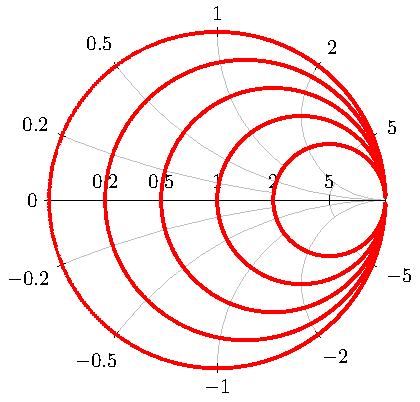
\includegraphics[width=5cm]{fig4-3.pdf}
          \caption{归一化电阻圆}
        \end{figure}
      \end{column}
      \begin{column}{0.55\linewidth}
        \begin{empheq}[box=\widefbox]{align*}
          \left(\Gamma_{\mathrm{Re}}-\frac{r}{r+1}\right)^2+\Gamma_{\mathrm{Im}}^2=\frac{1}{(r+1)^2}
        \end{empheq}
      \end{column}
    \end{columns}}
\end{frame}

\begin{frame}{Smith圆图的基本构成}
  电阻圆始终和直线$\Gamma_r=1$相切
  \begin{columns}
    \begin{column}{0.42\linewidth}
      \begin{figure}
        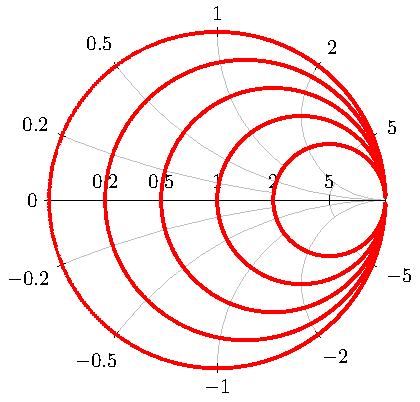
\includegraphics[width=4.55cm]{fig4-3.pdf}
        \caption{归一化电阻圆}
      \end{figure}
    \end{column}
    \begin{column}{0.58\linewidth}
      \begin{tabular}{|c|c|c|c|}
        \hline
        \multirow{2}*{$r$}                       &
        \multicolumn{2}{c|}{\footnotesize{圆心坐标}} &
        \multirow{2}*{\footnotesize{半径} $\left(\frac{1}{1+r}\right)$}                            \\ \cline{2-3}
                                                 & $\Gamma_r=\frac{r}{1+r}$ & $\Gamma_i=0$       \\ \hline
        0                                        & 0                        & 0            & 1   \\ \hline
        1                                        & 1/2                      & 0            & 1/2 \\ \hline
        2                                        & 2/3                      & 0            & 1/3 \\ \hline
      \end{tabular}
    \end{column}
  \end{columns}
  \begin{empheq}[box=\widefbox]{align*}
    \left(\Gamma_{\mathrm{Re}}-\frac{r}{r+1}\right)^2+\Gamma_{\mathrm{Im}}^2=\frac{1}{(r+1)^2}
  \end{empheq}
\end{frame}

\begin{frame}{Smith圆图的基本构成}
  电抗圆圆心坐标和半径
  \begin{empheq}[box=\widefbox]{align*}
    (\Gamma_{\mathrm{Re}}-1)^2+\left(\Gamma_{\mathrm{Im}}-\frac{1}{x}\right)^2=\left(\frac{1}{x}\right)^2
  \end{empheq}
  \begin{columns}
    \begin{column}{0.58\linewidth}
      \begin{tabular}{|c|c|c|c|}
        \hline
        \multirow{2}*{$x$}                       &
        \multicolumn{2}{c|}{\footnotesize{圆心坐标}} &
        \multirow{2}*{\footnotesize{半径} $\left(\frac{1}{x}\right)$}                               \\ \cline{2-3}
                                                 & $\Gamma_r=1$ & $\Gamma_i=\frac{1}{x}$          \\ \hline
        0                                        & 1            & \infty                 & \infty \\ \hline
        \pm0.5                                   & 1            & \pm2                   & 2      \\ \hline
        \pm1                                     & 1            & \pm1                   & 1      \\ \hline
      \end{tabular}
    \end{column}
    \begin{column}{0.42\linewidth}
      \begin{figure}
        \includegraphics[width=4.55cm]{fig4-4.pdf}
        \caption{归一化电抗圆}
      \end{figure}
    \end{column}
  \end{columns}
\end{frame}

\begin{frame}{Smith圆图的基本构成}
  将等电阻圆和等电抗圆绘制在同一张图上,得到阻抗圆图。
  \centering
  \includegraphics[width=8cm]{fig4-5.pdf}
\end{frame}

\begin{frame}{Smith圆图的特点}
  \begin{columns}
    \begin{column}{0.4\linewidth}
      \textbf{阻抗圆图有如下几个特点}
      \begin{itemize}
        \item 圆图上有三个特殊点:
              \footnotesize{\textbf{匹配点}(O点)\\
              其坐标为(0,0)\\
              $r=1,x=0$ \\
              $\lvert\Gamma\rvert=0,\rho=1$\\
              \textbf{短路点}(C点)\\
              其坐标为(-1,0)\\
              $r=0,x=0,\lvert\Gamma\rvert=1$ \\
              $\rho=\infty,\phi=\pi$ \\
              \textbf{开路点}(D点)\\
              其坐标为(1,0)\\
              $r=\infty,x=\infty,\lvert\Gamma\rvert=1$ \\
              $\rho=\infty,\phi=0$}
      \end{itemize}

    \end{column}
    \begin{column}{0.6\linewidth}
      \only<1>{\includegraphics[width=7cm]{MatchShortOpen1.pdf}}
      \only<2>{\includegraphics[width=7cm]{MatchShortOpen2.pdf}}
      \only<3>{\includegraphics[width=7cm]{MatchShortOpen3.pdf}}
    \end{column}
  \end{columns}
\end{frame}

\begin{frame}{Smith圆图的特点}
  \begin{columns}
    \begin{column}{0.4\linewidth}
      \begin{itemize}
        \item 圆图上有三条特殊线:
              \footnotesize{圆图上实轴为$x=0$的轨迹,\\
                \textbf{正半实轴}为电压波腹点的轨迹,线上$R$值为驻波比读数。\\
                \textbf{负半实轴}为电压波节点的轨迹,线上的$R$值为行波系数$K$的读数。\\
                \textbf{最外面的单位圆}为$R=0$的纯电抗轨迹,即为$\lvert\Gamma\rvert=1$的全反射系数圆的轨迹.\\}
        \item 圆上有两个特殊面
              \footnotesize{圆图实轴以上的上半平面是\textbf{感性}阻抗的轨迹;实轴以下的下半平面是\textbf{容性}阻抗的轨迹。}
      \end{itemize}
    \end{column}
    \begin{column}{0.6\linewidth}
      \only<1>{\includegraphics[width=7cm]{bofubojie1.pdf}}
      \only<2>{\includegraphics[width=7cm]{bofubojie2.pdf}}
      \only<3>{\includegraphics[width=7cm]{bofubojie3.pdf}}
    \end{column}
  \end{columns}
\end{frame}

\begin{frame}{Smith圆图的特点}
  \begin{columns}
    \begin{column}{0.4\linewidth}
      \begin{itemize}
        \item \footnotesize{圆图上有两个旋转方向,在传输线上向负载方向移动时,则在圆图上沿等反射系数圆逆时针方向旋转;反之,在传输线上向波源方向移动时,
                则在圆图上沿等反射系数圆顺时针方向旋转。}
        \item \footnotesize{圆图上任意一点对应四个参量:$x$,$r$,$\lvert\Gamma\rvert$和$\phi$,知道前两个参量或后两个参量
                均可确定该点在圆图上的位置。}
        \item \footnotesize{若传输线上某一位置对应于圆图上的A点,则A点的读数即为该位置的输入阻抗归一化值$r=\mathrm{j}x$;若关
                于O点的A点对称点为B点,则B点的读数即为该位置的输入导纳归一化值$g+\mathrm{j}b$。}
      \end{itemize}
    \end{column}

    \begin{column}{0.6\linewidth}
      \includegraphics[width=7cm]{xuanxiang.pdf}
    \end{column}
    
  \end{columns}
\end{frame}

\begin{frame}{Smith圆图的特点}
  \textbf{使用圆图应注意以下特点}\\
  \begin{columns}
    \begin{column}{0.4\linewidth}
      \begin{itemize}
        \item \footnotesize{当圆图作为阻抗圆图时,相角为0的反射系数位于OD上,相角增大,反射系数矢量沿逆时针方向转动;当圆图作为
              导纳圆图时,相角为0的反射系数位于OC上,相角增大,反射系数矢量仍沿逆时针方向转动。}
        \item \footnotesize{与阻抗圆图相反,作为导纳圆图使用时,D点为短路点,C点为开路点,线段OD为电压波节点归一化阻抗的轨迹,线
              段OC为电压波腹点归一化阻抗的轨迹}
        \item \footnotesize{$z(d)$与$y(d)$在同一反射系数圆上,相应位置差$180^{\circ}$}
      \end{itemize}
    \end{column}
    \begin{column}{0.6\linewidth}
      \includegraphics[width=7cm]{Z_Yyuantu.png}
    \end{column}
  \end{columns}
\end{frame}

\begin{frame}{Smith圆图的应用}
  Smith圆图的基本功能
  \begin{center}
    \begin{tabular}{|c|c|}
      \hline
      1 & 已知阻抗$Z$,求导纳$Y$(或逆问题)                  \\
      \hline
      2 & 已知阻抗$Z$,求反射系数$\Gamma$和$\rho$(或逆问题)    \\
      \hline
      3 & 已知阻抗$Z$和$\phi$求输入阻抗$Z_{in}$(或逆问题)     \\
      \hline
      4 & 已知驻波比和最小点$d_{\mathrm{min}}$,求$Z_{in}$ \\
      \hline
    \end{tabular}
  \end{center}
\end{frame}

\begin{frame}{Smith圆图的应用}
  例1 \quad 特性阻抗$Z_0=50\Omega$,负载阻抗$Z_L=100+j50\Omega$,求距负载$0.24\lambda$处输入阻抗。\\
  解:归一化负载阻抗$z_L=2+\mathrm{j}1$\\
  \begin{columns}
    \begin{column}{0.4\linewidth}
      1)\quad 向电源方向旋转$0.213\lambda$
      \begin{flalign*}
        \phi=\arctan(1/2)                         &  & \\
        \frac{2\pi}{\lambda/2}=\frac{\pi-\phi}{l} &  & \\
        l =(\pi-0.4636)\lambda/4\pi               &  & \\
        =0.213\lambda                             &  &
      \end{flalign*}
      2)\quad 旋转$0.24\lambda$到$z_{in}$
      \begin{align*}
        z_{in}=0.42-j0.25\rightarrow\times 50 \\
        \rightarrow 21-j12.5\Omega
      \end{align*}
    \end{column}
    \begin{column}{0.6\linewidth}

      \only<1>{\includegraphics[width=6.5cm]{SCexample1-eps-converted-to.pdf}}
      \only<2>{\includegraphics[width=6.5cm]{SCexample2-eps-converted-to.pdf}}
      \only<3>{\includegraphics[width=6.5cm]{SCexample3-eps-converted-to.pdf}}
      \only<4>{\includegraphics[width=6.5cm]{SCexample4-eps-converted-to.pdf}}
      \only<5>{\includegraphics[width=6.5cm]{SCexample5-eps-converted-to.pdf}}
      \only<6>{\includegraphics[width=6.5cm]{SCexample6-eps-converted-to.pdf}}
      \only<7>{\includegraphics[width=6.5cm]{SCexample7-eps-converted-to.pdf}}
      \only<8>{\includegraphics[width=6.5cm]{SCexample8-eps-converted-to.pdf}}
      \only<9>{\includegraphics[width=6.5cm]{SCexample9-eps-converted-to.pdf}}
      \only<10>{\includegraphics[width=6.5cm]{SCexample10-eps-converted-to.pdf}}
      \only<11>{\includegraphics[width=6.5cm]{SCexample11-eps-converted-to.pdf}}

      %\only<1>{\includegraphics[width=6cm]{SCexample1.eps}}
    \end{column}
  \end{columns}
\end{frame}

\begin{frame}{Smith圆图的应用}
  例2 \quad 已知无耗传输线的特征阻抗为$50\Omega$,长度为$0.1\lambda$,终端短路,求输入阻抗。
  \begin{columns}
    \begin{column}{0.4\linewidth}
      1)\quad 先找出终端短路点$S$\\
      2)\quad 向源方向旋转$0.1\lambda$,到圆图上$A$点,读出$x=0.72$
      \begin{flalign*}
        Z_{in}=Z_0z_{in}&=50\times\mathrm{j}0.72\\
        &=\mathrm{j}36\Omega
      \end{flalign*}
    \end{column}
    \begin{column}{0.6\linewidth}
      \only<1>{\includegraphics[width=6.5cm]{fig4-11-1.pdf}}
      \only<2>{\includegraphics[width=6.5cm]{fig4-11-2.pdf}}
      \only<3>{\includegraphics[width=6.5cm]{fig4-11-3.pdf}}
      \only<4>{\includegraphics[width=6.5cm]{fig4-11-4.pdf}}
      \only<5>{\includegraphics[width=6.5cm]{fig4-11-5.pdf}}
      \only<6>{\includegraphics[width=6.5cm]{fig4-11-6.pdf}}
      \only<7>{\includegraphics[width=6.5cm]{fig4-11-7.pdf}}
    \end{column}
  \end{columns}
\end{frame}

\begin{frame}{Smith圆图的应用}
  例3 \quad 已知无耗传输线的特征阻抗为$Z_0=50\Omega$,端接负载阻抗为$Z_L=(85+\mathrm{j}30)\Omega$,利用圆图求驻波比。
  \begin{columns}
    \begin{column}{0.4\linewidth}
      1)\quad 首先对负载归一化
      \begin{flalign*}
        z_L=\frac{Z_L}{Z_0}=1.7+\mathrm{j}0.6
      \end{flalign*}
      2)\quad 在$Smith$圆图中确定负载位置$A$点:$r=1.7,x=0.6$,并画出负载所在的等反射系数圆\\
      3)\quad 由图读出与等反射系数圆相切的电阻圆的$r$值即为驻波比 $\rho=2.0$
    \end{column}
    \begin{column}{0.6\linewidth}
      \only<1>{\includegraphics[width=7cm]{fig4-12-1.pdf}}
      \only<2>{\includegraphics[width=7cm]{fig4-12-2.pdf}}
      \only<3>{\includegraphics[width=7cm]{fig4-12-3.pdf}}
      \only<4>{\includegraphics[width=7cm]{fig4-12-4.pdf}}
      \only<5>{\includegraphics[width=7cm]{fig4-12-5.pdf}}
      \only<6>{\includegraphics[width=7cm]{fig4-12-6.pdf}}
      \only<7>{\includegraphics[width=7cm]{fig4-12-7.pdf}}
    \end{column}
  \end{columns} 
\end{frame}

\begin{frame}{Smith圆图的应用}
  例4 \quad 已知传输线长$l=25m$,特征阻抗为$100\Omega$,端接负载阻抗为$Z_L=(100-\mathrm{j}200)\Omega$,信号源频率为$f=10MHz$,利用Smith圆图求输入阻抗及导纳。
  \begin{columns}
    \begin{column}{0.4\linewidth}
      1)\quad 首先对负载归一化
      \begin{flalign*}
        z_L=\frac{Z_L}{Z_0}=1-\mathrm{j}2
      \end{flalign*}
      2)\quad 图中定位$A$点:$r=1,x=-2$,由题知$\lambda=30m$,传输线长$l=25m$,所以由$A$点沿等反射系数圆顺时针转动
      \begin{flalign*}
        \frac{l}{\lambda}=\frac{5}{6}=0.833=0.5+0.333
      \end{flalign*}
      到输入阻抗点,而
    \end{column}
    \begin{column}{0.6\linewidth}
      \only<1>{\includegraphics[width=6.5cm]{fig4-13-1.pdf}}
      \only<2>{\includegraphics[width=6.5cm]{fig4-13-2.pdf}}
      \only<3>{\includegraphics[width=6.5cm]{fig4-13-3.pdf}}
      \only<4>{\includegraphics[width=6.5cm]{fig4-13-4.pdf}}
      \only<5>{\includegraphics[width=6.5cm]{fig4-13-5.pdf}}
    \end{column}
  \end{columns}
\end{frame}


\begin{frame}{Smith圆图的应用}
  \begin{columns}
    \begin{column}{0.4\linewidth}
      \begin{flalign*}
        2\beta l=4\pi\frac{5}{6}=2\pi+\frac{4}{3}\pi
      \end{flalign*}
      3)\quad 由负载对应的$A$点先沿等反射系数圆顺时针转动0.5刻度,对应$2\pi$,再转$\dfrac{4}{3}\pi$,对应0.333刻度,到达$B$点,$B$点即为输入阻抗点。从图中读出该点读数:$0.45+\mathrm{j}1.2$,反归一化,得到输入阻抗
      \begin{flalign*}
        Z_{in}&=(0.45+\mathrm{j}1.2)\times 100\\
        &=(45+\mathrm{j}120)\Omega
      \end{flalign*}  
    \end{column}
    \begin{column}{0.6\linewidth}
      \includegraphics[width=6.5cm]{fig4-13-6.pdf}
    \end{column}
  \end{columns}
\end{frame}

\begin{frame}{Smith圆图的应用}
  \begin{columns}
    \begin{column}{0.4\linewidth}
      4)\quad 再由$OB$反向延长到$C$点,为归一化导纳点,读出该点的值为$y_{in}=0.27-\mathrm{j}0.73$,所以输入导纳为
      \begin{flalign*}
        Y_{in}&=(0.27-\mathrm{j}0.73)/100\\
        &=0.0027-\mathrm{j}0.0073
      \end{flalign*}
    \end{column}
    \begin{column}{0.6\linewidth}
      \includegraphics[width=6.5cm]{fig4-13-7.pdf}
    \end{column}
  \end{columns}
\end{frame}

\begin{frame}{Smith圆图的应用}
  例5 \quad 如图所示,已知一无耗传输线的特性阻抗为$50\Omega$,驻波比$\rho=3$,相邻两个电压最小值点的距离为$0.2m$,距离负载最近的电压驻波最小值点距负载$0.05m$,求:(1)负载处反射系数;(2)负载阻抗
  \begin{columns}
    \begin{column}{0.4\linewidth}
      由题可知$\lambda/2=0.2m$,所以$\lambda=0.4m$,由已知条件有
      \begin{flalign*}
        \rho=\lvert V_{\mathrm{max}}\rvert / \lvert V_{\mathrm{min}}\rvert = 3
      \end{flalign*}
      因为$\rho=\dfrac{1+\lvert \Gamma \rvert}{1-\lvert \Gamma \rvert}$,所以
      \begin{flalign*}
        \lvert \Gamma_L \rvert = \lvert \Gamma \rvert = \frac{\rho-1}{\rho+1}=\frac{1}{2}
      \end{flalign*}
      1)\quad 绘出等反射系数圆
      
    \end{column}
    \begin{column}{0.6\linewidth}
      \includegraphics[width=6.5cm]{fig4-16-1.pdf}
    \end{column}
  \end{columns}
\end{frame}

\begin{frame}{Smith圆图的应用}
  \begin{columns}
    \begin{column}{0.4\linewidth}
      2)\quad 第一个最小值点处反射波相位为$-\pi$,对应$E$点,延长$OE$,与单位圆交于点$H$,由$H$点向负载(逆时针)转动$\dfrac{d_{\mathrm{min}}}{\lambda}=\dfrac{1}{8}$刻度,得到点$F$。等反射系数圆与$OF$的交点
      为$G$点。由$G$点读出的即为归一化负载阻抗$0.6-\mathrm{j}0.8$,进行反归一化,得到负载阻抗为$(0.6-\mathrm{j}0.8)\times 50=30-\mathrm{j}40$\\
      3)\quad 由$G$点读出反射系数为:
      \begin{flalign*}
        \Gamma_L=-\mathrm{j}0.5
      \end{flalign*}
    \end{column}
    \begin{column}{0.6\linewidth}
      \only<1>{\includegraphics[width=6.5cm]{fig4-16-2.pdf}}
      \only<2>{\includegraphics[width=6.5cm]{fig4-16-3.pdf}}
      \only<3>{\includegraphics[width=6.5cm]{fig4-16-4.pdf}}
    \end{column}
  \end{columns}
\end{frame}

\begin{frame}{Smith圆图的应用}
  例6 \quad 已知一无耗传输线的特征阻抗为$50\Omega$,端接负载阻抗$Z_L$,驻波电压最大值和最小值分别为$V_{\mathrm{max}}=2.5V$和$V_{\mathrm{min}}=1V$,相邻两个电压最小值点距离为$0.05m$。当负载处由解纯电阻$R(R<Z_0)$
  改为接负载$Z_L$时,电压最小值向源方向移动$1.25cm$,求负载阻抗$Z_L$。
  \begin{columns}
    \begin{column}{0.4\linewidth}
      1)\quad 驻波比
      \begin{flalign*}
        \rho=\lvert V_{\mathrm{max}}\rvert/\lvert V_{\mathrm{min}}\rvert=2.5
      \end{flalign*}
      2)\quad 相邻两个电压最小值点的距离为0.05m,即半波长$\lambda/2=0.05m$,即$\lambda=0.1m$,从而移动$1.25cm$为$\lambda/8$。\\
      3)\quad 当负载处由纯电阻换为接负载$Z_L$时,电压最小值向源方向移动$\lambda/8$,相当于纯电阻点向源移动$\lambda/8$\\  
    \end{column}
    \begin{column}{0.6\linewidth}
      %TODO:
    \end{column}
  \end{columns}
\end{frame}

\begin{frame}{Smith圆图的应用}
  \begin{columns}
    \begin{column}{0.4\linewidth}
      4)\quad 端接负载$Z_L$的传输系统的$A$点输入阻抗为$R$,由$\rho=2.5=r$可以确定等反射系数圆$\lvert\Gamma\rvert$\\
      5)\quad 由于端接纯电阻时对应电压最小值,$R$处电压最小,$r=R/Z_0<1$,说明纯电阻点在横轴的负半轴上$E$点,
    \end{column}
    \begin{column}{0.6\linewidth}
      %TODO:
    \end{column}
  \end{columns}
\end{frame}

\begin{frame}
  \begin{columns}
    \begin{column}{0.4\linewidth}
      6)\quad 对于端接负载$Z_L$的传输系统,对应圆图上点$E$向负载逆时针旋转$\lambda/8$到点$G$,即得到$Z_L$。从圆图上读出归一化阻抗为
      $0.69-\mathrm{j}0.72$,所以负载阻抗为
      \begin{flalign*}
        Z_L&=0.69-\mathrm{j}0.72\times 50\\
        &=(34.5-\mathrm{j}36)\Omega
      \end{flalign*}
      7)\quad 导纳为(对应F点)
      \begin{flalign*}
        Y_L=1/Z_L=0.02006\angle 46.23^{\circ} S
      \end{flalign*}
    \end{column}
    \begin{column}{0.6\linewidth}
      
    \end{column}
  \end{columns}
\end{frame}

\begin{frame}{Smith导纳圆图}
  \begin{itemize}
    \item 导纳圆图
  \end{itemize}
  %TODO:
\end{frame}

\subsection{阻抗匹配}
\begin{frame}{阻抗匹配}

\end{frame}

\subsection{支节匹配器}
\begin{frame}{支节匹配器}

\end{frame}

\subsection{$\lambda/4$ 阻抗变换器}
\begin{frame}{$\lambda/4$ 阻抗变换器}

\end{frame}

\subsection{小反射理论}
\begin{frame}{小反射理论}

\end{frame}

\subsection{二项式(最大平坦特性)多节阻抗变换器}
\begin{frame}{二项式(最大平坦特性)多节阻抗变换器}

\end{frame}

\subsection{切比雪夫(等波纹特性)多节阻抗变换器}
\begin{frame}{切比雪夫(等波纹特性)多节阻抗变换器}

\end{frame}

\subsection{渐变传输线}
\begin{frame}{渐变传输线}

\end{frame}

\section{第5章\quad 微波网络理论与分析}
\begin{frame}{第5章\quad 微波网络基础}

\end{frame}

\subsection{微波网络概念及等效关系}
\begin{frame}{微波网络概念及等效关系}

\end{frame}

\subsection{微波网络参量}
\begin{frame}{微波网络参量}

\end{frame}

\subsection{微波网络参量的性质}
\begin{frame}{微波网络参量的性质}

\end{frame}

\subsection{二端口微波网络的工作特性参量}
\begin{frame}{二端口微波网络的工作特性参量}

\end{frame}

\subsection{微波网络的组合}
\begin{frame}{微波网络的组合}

\end{frame}

\subsection{二端口网络的等效电路}
\begin{frame}{二端口网络的等效电路}

\end{frame}

\subsection{信号流图分析及其应用}
\begin{frame}{信号流图分析及其应用}

\end{frame}


\section{第6章\quad 实用微波传输线与波导}
\begin{frame}{第6章\quad 实用微波传输线与波导}
    \begin{itemize}
        \item 微波工程分析方法
              \begin{itemize}
                  \item 场论的方法
                  \item 网络的方法
              \end{itemize}
    \end{itemize}
    \begin{itemize}
        \item 传输线理论 $\Longrightarrow$ 波导
              \begin{itemize}
                  \item 当其他人或物靠近双导线时会产生较大影响。这说明,传输线与外界有能量交换,它带来的直接问题是能量损失和工作不稳定。就其原因是\textbf{开放(Open)}造成的特点
              \end{itemize}
    \end{itemize}
\end{frame}

\begin{frame}{第6章\quad 实用微波传输线与波导}
    \begin{itemize}
        \item 波导(Waveguide)构成
    \end{itemize}
    双导线两侧连续加对称$\lambda/4$支节,直到构成封闭(Closed)电路为止。如果其导线的宽度是$W$,则波导宽边
    \begin{align*}
        a=W+2\cdot \frac{\lambda}{4}=W+\frac{\lambda}{2} \\
        a\geqslant \lambda/2 或 \lambda\leqslant 2a
    \end{align*}
    这构成了波导传输的第一个约束条件 \\
    \centering
    \includegraphics[width=6cm]{fig6-0.png}
\end{frame}

\begin{frame}{第6章\quad 实用微波传输线与波导}
    \begin{itemize}
        \item 波导一般解的出发点和假定条件\\
              波导一般解的出发点是频域Maxwell方程组
              \begin{align}
                  \begin{cases}
                      \nabla\times\vec{H}=\rm{j}\omega\epsilon\vec{E} \\
                      \nabla\times\vec{E}=-\rm{j}\omega\mu\vec{H}     \\
                      \nabla\cdot\vec{E}=0                            \\
                      \nabla\cdot\vec{H}=0
                  \end{cases}\label{eqn6-1}
              \end{align}
              波导假定条件
              \begin{columns}
                  \begin{column}{0.5\linewidth}
                      \begin{itemize}
                          \item 波导均匀条件:假定横截面不随$z$而变化
                          \item 媒质均匀条件:波导内部$\epsilon,\mu$均匀,波导内壁$\sigma$无限大
                          \item 无源条件:波导内$\rho,\vec{J}\equiv 0$
                          \item 无限条件:波导在$z$方向无限长
                      \end{itemize}
                  \end{column}
                  \begin{column}{0.5\linewidth}
                      \includegraphics[width=5cm]{fig6-1.png}
                  \end{column}
              \end{columns}
    \end{itemize}
\end{frame}

\subsection{传输线的一般传输特性}
\begin{frame}{传输线的一般传输特性}
    (\ref{eqn6-1})第二式两边取旋度
    \begin{align*}
        \nabla\times\nabla\times\vec{E} & =\nabla(\nabla\cdot\vec{E})-\nabla^2\vec{E}=-\rm{j}\omega\mu\nabla\times\vec{H} \\
                                        & =\omega^2\mu\epsilon\vec{E}=k^2\vec{E}
    \end{align*}
    得到波动方程
    \begin{align}
        \begin{cases}
            \nabla^2\vec{E}+k^2\vec{E}=0 \\
            \nabla^2\vec{H}+k^2\vec{H}=0 \\
        \end{cases}\label{eqn6-2}
    \end{align}
\end{frame}

\subsection{矩形波导}
\begin{frame}{矩形波导}

\end{frame}

\subsection{圆波导}
\begin{frame}{圆波导}

\end{frame}

\subsection{同轴线}
\begin{frame}{同轴线}

\end{frame}

\subsection{平面传输线}
\begin{frame}{平面传输线}
    上世纪六十年代以来,在微波工程和微波技术上,出现了一次不小的革命,即所谓MIC(Microwave Integrated Circuit)微波集成电路——HMIC、MMIC。其特色是体积小、功能多、频带宽,但承受功率小。因此被广泛应用于接收机和小功率元件中,并都传输TEM波。\\
    作为这一革命的“过渡人物”是带状线(Stripline)。它可以看作是同轴线的变形。
\end{frame}







\section{第七章\quad 微波谐振器}
\begin{frame}{第七章\quad 微波谐振器}

\end{frame}

\subsection{微波谐振器的基本特性与参数}
\begin{frame}{微波谐振器的基本特性与参数}

\end{frame}

\subsection{串联和并联谐振电路}
\begin{frame}{串联和并联谐振电路}

\end{frame}

\subsection{传输线谐振器}
\begin{frame}{传输线谐振器}

\end{frame}

\subsection{金属波导谐振腔}
\begin{frame}{金属波导谐振腔}

\end{frame}

\subsection{介质谐振器}
\begin{frame}{介质谐振器}

\end{frame}

\subsection{法布里-珀罗谐振器}
\begin{frame}{法布里-珀罗谐振器}

\end{frame}

\subsection{谐振器的激励}
\begin{frame}{谐振器的激励}

\end{frame}

\subsection{微波谐振腔的微扰理论}
\begin{frame}{微波谐振腔的微扰理论}

\end{frame}

\section{第八章\quad 常用微波元件}
\begin{frame}{第八章\quad 常用微波元件}

\end{frame}

\subsection{一端口元件}
\begin{frame}{一端口元件}

\end{frame}

\subsection{二端口元件}
\begin{frame}{二端口元件}

\end{frame}

\subsection{三端口元件}
\begin{frame}{三端口元件}

\end{frame}

\subsection{四端口元件}
\begin{frame}{四端口元件}

\end{frame}

\subsection{微波周期结构}
\begin{frame}{微波周期结构}

\end{frame}

\section{第九章\quad 微波铁氧体元件}
\begin{frame}{第九章\quad 微波铁氧体元件}

\end{frame}

\subsection{微波铁氧体的基本特性}
\begin{frame}{微波铁氧体的基本特性}

\end{frame}

\subsection{铁氧体媒质中的平面波}
\begin{frame}{铁氧体媒质中的平面波}

\end{frame}

\subsection{铁氧体加载矩形波导}
\begin{frame}{铁氧体加载矩形波导}

\end{frame}

\subsection{微波铁氧体隔离器}
\begin{frame}{微波铁氧体隔离器}

\end{frame}

\subsection{微波铁氧体相移器}
\begin{frame}{微波铁氧体相移器}

\end{frame}

\subsection{微波铁氧体环行器}
\begin{frame}{微波铁氧体环行器}

\end{frame}

\end{document}
